% ONE SHEET / EIGHT PAGES — single-file LaTeX mini-zine
% Print:   pdflatex mini-zine.tex  (run twice to resolve page positions)
% Preview: pdflatex -jobname=mini-zine-preview "\def\ZinePreview{1}% ONE SHEET / EIGHT PAGES — single-file LaTeX mini-zine
% Print:   pdflatex mini-zine.tex  (run twice to resolve page positions)
% Preview: pdflatex -jobname=mini-zine-preview "\def\ZinePreview{1}% ONE SHEET / EIGHT PAGES — single-file LaTeX mini-zine
% Print:   pdflatex mini-zine.tex  (run twice to resolve page positions)
% Preview: pdflatex -jobname=mini-zine-preview "\def\ZinePreview{1}% ONE SHEET / EIGHT PAGES — single-file LaTeX mini-zine
% Print:   pdflatex mini-zine.tex  (run twice to resolve page positions)
% Preview: pdflatex -jobname=mini-zine-preview "\def\ZinePreview{1}\input{mini-zine.tex}"
% Clean:   pdflatex -jobname=mini-zine-clean "\def\ZineNoGuides{1}\input{mini-zine.tex}"
% US Letter: uncomment \def\ZineLetter{1} below (or define it on the command line).
% Layout reference: https://github.com/krthr/fanzines.app#geometra-e-imposicin
% Print one-sided in landscape at Actual Size (100%), not "Fit".
% Crease the 4 x 2 grid. Cut ONLY the solid center segment between the
% first and third vertical folds. Fold lengthwise, print facing out, then
% push the two ends together; flatten the resulting cross into a booklet.
% \ZinePage{0} is the front, 1--6 are inside, and 7 is the back.
% Images: \includegraphics[width=\linewidth,height=30mm,keepaspectratio]{photo.jpg}

\RequirePackage{fix-cm}
\documentclass[10pt]{article}
\usepackage{geometry}
\usepackage{tikz}
\usepackage{graphicx}

% \def\ZineLetter{1}

\newlength\SheetW \newlength\SheetH
\newlength\PanelW \newlength\PanelH
\newlength\SafeMargin \setlength\SafeMargin{6mm}
\newlength\InnerW \newlength\InnerH
\ifdefined\ZineLetter
  \setlength\SheetW{11in} \setlength\SheetH{8.5in}
\else
  \setlength\SheetW{297mm} \setlength\SheetH{210mm}
\fi
\setlength\PanelW{\dimexpr\SheetW/4\relax}
\setlength\PanelH{\dimexpr\SheetH/2\relax}
\setlength\InnerW{\dimexpr\PanelW-2\SafeMargin\relax}
\setlength\InnerH{\dimexpr\PanelH-2\SafeMargin\relax}
\ifdefined\ZinePreview
  \geometry{paperwidth=\PanelW,paperheight=\PanelH,margin=0pt}
\else
  \geometry{paperwidth=\SheetW,paperheight=\SheetH,margin=0pt}
\fi
\pagestyle{empty}
\setlength\parindent{0pt}

\definecolor{ink}{HTML}{172839}
\definecolor{accent}{HTML}{B34327}
\definecolor{muted}{HTML}{545E6A}
\definecolor{tint}{HTML}{F1E3D6}

% ---- Edit these eight blocks, in reading order. ----
\newcommand\ZinePage[2]{\expandafter\long\expandafter\gdef\csname zinepage#1\endcsname{#2}}
\newcommand\Kicker[1]{\textcolor{accent}{\sffamily\bfseries\scriptsize #1}\par\smallskip}
\newcommand\Headline[1]{{\sffamily\bfseries\LARGE #1\par}\medskip}
\newcommand\PageNo[1]{\par\vspace{6mm}{\color{muted}\sffamily\scriptsize #1\par}}

\ZinePage{0}{
  \Kicker{A ONE-SHEET MINI-ZINE}
  \vspace{7mm}
  {\sffamily\bfseries\fontsize{27}{30}\selectfont
  One sheet.\par Eight pages.\par}
  \vspace{6mm}
  {\color{accent}\rule{20mm}{1.3pt}}\par\medskip
  Write it in order.\par Fold it into a book.
}
\ZinePage{1}{
  \Kicker{01 / WRITE}
  \Headline{Start here}
  Each page lives in a \texttt{\string\ZinePage} block. Write the cover, six inside pages, and the back in reading order.
  \medskip\par
  LaTeX takes care of flipping and rearranging them on the print sheet.
  \PageNo{01}
}
\ZinePage{2}{
  \Kicker{02 / DESIGN}
  \Headline{Make it yours}
  Use normal LaTeX: headings, lists, math, photos, or drawings.
  \begin{center}
    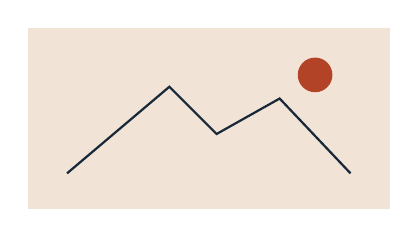
\begin{tikzpicture}[x=1cm,y=1cm]
      \fill[tint] (0,0) rectangle (4.6,2.3);
      \draw[ink,thick] (.5,.45) -- (1.8,1.55) -- (2.4,.95) -- (3.2,1.4) -- (4.1,.45);
      \fill[accent] (3.65,1.7) circle (2.2mm);
    \end{tikzpicture}
  \end{center}
  Replace the drawing with a photo or keep the page all text.
  \PageNo{02}
}
\ZinePage{3}{
  \Kicker{03 / PRINT}
  \Headline{One side only}
  Print the landscape sheet at \textbf{Actual Size (100\%)} on A4, or select US Letter in the source first.
  \medskip\par
  The top row is upside down on purpose.
  \PageNo{03}
}
\ZinePage{4}{
  \Kicker{04 / CREASE}
  \Headline{Make eight panels}
  Crease the sheet once down its length and three times across its width, following the dashed guides.
  \medskip\par
  Unfold it flat before making the cut.
  \PageNo{04}
}
\ZinePage{5}{
  \Kicker{05 / CUT}
  \Headline{Just one slit}
  Cut along the \textbf{solid middle line only}: start at the first vertical fold and stop at the third.
  \medskip\par
  Leave both outer sections attached.
  \PageNo{05}
}
\ZinePage{6}{
  \Kicker{06 / FOLD}
  \Headline{Push the ends in}
  Fold lengthwise with the print facing out. Push the two short ends toward each other until the slit opens into a diamond.
  \medskip\par
  Flatten the diamond into a cross, then wrap the panels until the front and back covers are on the outside.
  \PageNo{06}
}
\ZinePage{7}{
  \Kicker{BACK COVER}
  \vspace{15mm}
  {\sffamily\bfseries\LARGE Made to fold.\par}\medskip
  One sheet of paper.\par
  No staples or glue.\par
  \vspace{7mm}
  {\color{accent}\rule{20mm}{1.3pt}}
}

% ---- Imposition engine. You shouldn't need to edit below this line. ----
\newsavebox\PanelContent
\newcommand\PanelBox[1]{%
  \begin{lrbox}{\PanelContent}%
    \begin{minipage}{\InnerW}%
      \raggedright\normalfont\normalsize\color{ink}%
      \setlength\parskip{3pt}%
      \csname zinepage#1\endcsname\par
    \end{minipage}%
  \end{lrbox}%
  \ifdim\dimexpr\ht\PanelContent+\dp\PanelContent\relax>\InnerH
    \PackageWarningNoLine{mini-zine}{Panel #1 exceeds the safe height; shorten the content}%
  \fi
  \begin{minipage}[c][\InnerH][t]{\InnerW}%
    \noindent\usebox\PanelContent\par
  \end{minipage}%
}
\newcommand\ZineSheet{%
  \null
  \begin{tikzpicture}[remember picture,overlay]
    \begin{scope}[shift={(current page.south west)},x=\PanelW,y=\PanelH]
      % Printed view, left to right: 6 5 4 3 up top; back front 1 2 below.
      \foreach \p [count=\i from 0] in {7,0,1,2}
        \node[inner sep=0pt,outer sep=0pt] at ({\i+.5},.5) {\PanelBox{\p}};
      \foreach \p [count=\i from 0] in {6,5,4,3}
        \node[inner sep=0pt,outer sep=0pt,rotate=180] at ({\i+.5},1.5) {\PanelBox{\p}};
      \ifdefined\ZineNoGuides\else
        \foreach \x in {1,2,3}
          \draw[muted!60,dashed,line width=.3pt] ([yshift=5mm]\x,0) -- ([yshift=-5mm]\x,2);
        \draw[muted!60,dashed,line width=.3pt] ([xshift=5mm]0,1) -- (1,1);
        \draw[muted!60,dashed,line width=.3pt] (3,1) -- ([xshift=-5mm]4,1);
        \draw[accent,line width=.65pt] (1,1) -- (3,1);
      \fi
    \end{scope}
  \end{tikzpicture}%
}
\newcommand\ZineReadPage[1]{%
  \null
  \begin{tikzpicture}[remember picture,overlay]
    \node[inner sep=0pt,outer sep=0pt] at (current page.center) {\PanelBox{#1}};
  \end{tikzpicture}%
}

\begin{document}
\ifdefined\ZinePreview
  \ZineReadPage{0}\newpage\ZineReadPage{1}\newpage
  \ZineReadPage{2}\newpage\ZineReadPage{3}\newpage
  \ZineReadPage{4}\newpage\ZineReadPage{5}\newpage
  \ZineReadPage{6}\newpage\ZineReadPage{7}
\else
  \ZineSheet
\fi
\end{document}
"
% Clean:   pdflatex -jobname=mini-zine-clean "\def\ZineNoGuides{1}% ONE SHEET / EIGHT PAGES — single-file LaTeX mini-zine
% Print:   pdflatex mini-zine.tex  (run twice to resolve page positions)
% Preview: pdflatex -jobname=mini-zine-preview "\def\ZinePreview{1}\input{mini-zine.tex}"
% Clean:   pdflatex -jobname=mini-zine-clean "\def\ZineNoGuides{1}\input{mini-zine.tex}"
% US Letter: uncomment \def\ZineLetter{1} below (or define it on the command line).
% Layout reference: https://github.com/krthr/fanzines.app#geometra-e-imposicin
% Print one-sided in landscape at Actual Size (100%), not "Fit".
% Crease the 4 x 2 grid. Cut ONLY the solid center segment between the
% first and third vertical folds. Fold lengthwise, print facing out, then
% push the two ends together; flatten the resulting cross into a booklet.
% \ZinePage{0} is the front, 1--6 are inside, and 7 is the back.
% Images: \includegraphics[width=\linewidth,height=30mm,keepaspectratio]{photo.jpg}

\RequirePackage{fix-cm}
\documentclass[10pt]{article}
\usepackage{geometry}
\usepackage{tikz}
\usepackage{graphicx}

% \def\ZineLetter{1}

\newlength\SheetW \newlength\SheetH
\newlength\PanelW \newlength\PanelH
\newlength\SafeMargin \setlength\SafeMargin{6mm}
\newlength\InnerW \newlength\InnerH
\ifdefined\ZineLetter
  \setlength\SheetW{11in} \setlength\SheetH{8.5in}
\else
  \setlength\SheetW{297mm} \setlength\SheetH{210mm}
\fi
\setlength\PanelW{\dimexpr\SheetW/4\relax}
\setlength\PanelH{\dimexpr\SheetH/2\relax}
\setlength\InnerW{\dimexpr\PanelW-2\SafeMargin\relax}
\setlength\InnerH{\dimexpr\PanelH-2\SafeMargin\relax}
\ifdefined\ZinePreview
  \geometry{paperwidth=\PanelW,paperheight=\PanelH,margin=0pt}
\else
  \geometry{paperwidth=\SheetW,paperheight=\SheetH,margin=0pt}
\fi
\pagestyle{empty}
\setlength\parindent{0pt}

\definecolor{ink}{HTML}{172839}
\definecolor{accent}{HTML}{B34327}
\definecolor{muted}{HTML}{545E6A}
\definecolor{tint}{HTML}{F1E3D6}

% ---- Edit these eight blocks, in reading order. ----
\newcommand\ZinePage[2]{\expandafter\long\expandafter\gdef\csname zinepage#1\endcsname{#2}}
\newcommand\Kicker[1]{\textcolor{accent}{\sffamily\bfseries\scriptsize #1}\par\smallskip}
\newcommand\Headline[1]{{\sffamily\bfseries\LARGE #1\par}\medskip}
\newcommand\PageNo[1]{\par\vspace{6mm}{\color{muted}\sffamily\scriptsize #1\par}}

\ZinePage{0}{
  \Kicker{A ONE-SHEET MINI-ZINE}
  \vspace{7mm}
  {\sffamily\bfseries\fontsize{27}{30}\selectfont
  One sheet.\par Eight pages.\par}
  \vspace{6mm}
  {\color{accent}\rule{20mm}{1.3pt}}\par\medskip
  Write it in order.\par Fold it into a book.
}
\ZinePage{1}{
  \Kicker{01 / WRITE}
  \Headline{Start here}
  Each page lives in a \texttt{\string\ZinePage} block. Write the cover, six inside pages, and the back in reading order.
  \medskip\par
  LaTeX takes care of flipping and rearranging them on the print sheet.
  \PageNo{01}
}
\ZinePage{2}{
  \Kicker{02 / DESIGN}
  \Headline{Make it yours}
  Use normal LaTeX: headings, lists, math, photos, or drawings.
  \begin{center}
    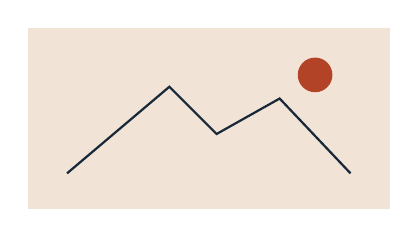
\begin{tikzpicture}[x=1cm,y=1cm]
      \fill[tint] (0,0) rectangle (4.6,2.3);
      \draw[ink,thick] (.5,.45) -- (1.8,1.55) -- (2.4,.95) -- (3.2,1.4) -- (4.1,.45);
      \fill[accent] (3.65,1.7) circle (2.2mm);
    \end{tikzpicture}
  \end{center}
  Replace the drawing with a photo or keep the page all text.
  \PageNo{02}
}
\ZinePage{3}{
  \Kicker{03 / PRINT}
  \Headline{One side only}
  Print the landscape sheet at \textbf{Actual Size (100\%)} on A4, or select US Letter in the source first.
  \medskip\par
  The top row is upside down on purpose.
  \PageNo{03}
}
\ZinePage{4}{
  \Kicker{04 / CREASE}
  \Headline{Make eight panels}
  Crease the sheet once down its length and three times across its width, following the dashed guides.
  \medskip\par
  Unfold it flat before making the cut.
  \PageNo{04}
}
\ZinePage{5}{
  \Kicker{05 / CUT}
  \Headline{Just one slit}
  Cut along the \textbf{solid middle line only}: start at the first vertical fold and stop at the third.
  \medskip\par
  Leave both outer sections attached.
  \PageNo{05}
}
\ZinePage{6}{
  \Kicker{06 / FOLD}
  \Headline{Push the ends in}
  Fold lengthwise with the print facing out. Push the two short ends toward each other until the slit opens into a diamond.
  \medskip\par
  Flatten the diamond into a cross, then wrap the panels until the front and back covers are on the outside.
  \PageNo{06}
}
\ZinePage{7}{
  \Kicker{BACK COVER}
  \vspace{15mm}
  {\sffamily\bfseries\LARGE Made to fold.\par}\medskip
  One sheet of paper.\par
  No staples or glue.\par
  \vspace{7mm}
  {\color{accent}\rule{20mm}{1.3pt}}
}

% ---- Imposition engine. You shouldn't need to edit below this line. ----
\newsavebox\PanelContent
\newcommand\PanelBox[1]{%
  \begin{lrbox}{\PanelContent}%
    \begin{minipage}{\InnerW}%
      \raggedright\normalfont\normalsize\color{ink}%
      \setlength\parskip{3pt}%
      \csname zinepage#1\endcsname\par
    \end{minipage}%
  \end{lrbox}%
  \ifdim\dimexpr\ht\PanelContent+\dp\PanelContent\relax>\InnerH
    \PackageWarningNoLine{mini-zine}{Panel #1 exceeds the safe height; shorten the content}%
  \fi
  \begin{minipage}[c][\InnerH][t]{\InnerW}%
    \noindent\usebox\PanelContent\par
  \end{minipage}%
}
\newcommand\ZineSheet{%
  \null
  \begin{tikzpicture}[remember picture,overlay]
    \begin{scope}[shift={(current page.south west)},x=\PanelW,y=\PanelH]
      % Printed view, left to right: 6 5 4 3 up top; back front 1 2 below.
      \foreach \p [count=\i from 0] in {7,0,1,2}
        \node[inner sep=0pt,outer sep=0pt] at ({\i+.5},.5) {\PanelBox{\p}};
      \foreach \p [count=\i from 0] in {6,5,4,3}
        \node[inner sep=0pt,outer sep=0pt,rotate=180] at ({\i+.5},1.5) {\PanelBox{\p}};
      \ifdefined\ZineNoGuides\else
        \foreach \x in {1,2,3}
          \draw[muted!60,dashed,line width=.3pt] ([yshift=5mm]\x,0) -- ([yshift=-5mm]\x,2);
        \draw[muted!60,dashed,line width=.3pt] ([xshift=5mm]0,1) -- (1,1);
        \draw[muted!60,dashed,line width=.3pt] (3,1) -- ([xshift=-5mm]4,1);
        \draw[accent,line width=.65pt] (1,1) -- (3,1);
      \fi
    \end{scope}
  \end{tikzpicture}%
}
\newcommand\ZineReadPage[1]{%
  \null
  \begin{tikzpicture}[remember picture,overlay]
    \node[inner sep=0pt,outer sep=0pt] at (current page.center) {\PanelBox{#1}};
  \end{tikzpicture}%
}

\begin{document}
\ifdefined\ZinePreview
  \ZineReadPage{0}\newpage\ZineReadPage{1}\newpage
  \ZineReadPage{2}\newpage\ZineReadPage{3}\newpage
  \ZineReadPage{4}\newpage\ZineReadPage{5}\newpage
  \ZineReadPage{6}\newpage\ZineReadPage{7}
\else
  \ZineSheet
\fi
\end{document}
"
% US Letter: uncomment \def\ZineLetter{1} below (or define it on the command line).
% Layout reference: https://github.com/krthr/fanzines.app#geometra-e-imposicin
% Print one-sided in landscape at Actual Size (100%), not "Fit".
% Crease the 4 x 2 grid. Cut ONLY the solid center segment between the
% first and third vertical folds. Fold lengthwise, print facing out, then
% push the two ends together; flatten the resulting cross into a booklet.
% \ZinePage{0} is the front, 1--6 are inside, and 7 is the back.
% Images: \includegraphics[width=\linewidth,height=30mm,keepaspectratio]{photo.jpg}

\RequirePackage{fix-cm}
\documentclass[10pt]{article}
\usepackage{geometry}
\usepackage{tikz}
\usepackage{graphicx}

% \def\ZineLetter{1}

\newlength\SheetW \newlength\SheetH
\newlength\PanelW \newlength\PanelH
\newlength\SafeMargin \setlength\SafeMargin{6mm}
\newlength\InnerW \newlength\InnerH
\ifdefined\ZineLetter
  \setlength\SheetW{11in} \setlength\SheetH{8.5in}
\else
  \setlength\SheetW{297mm} \setlength\SheetH{210mm}
\fi
\setlength\PanelW{\dimexpr\SheetW/4\relax}
\setlength\PanelH{\dimexpr\SheetH/2\relax}
\setlength\InnerW{\dimexpr\PanelW-2\SafeMargin\relax}
\setlength\InnerH{\dimexpr\PanelH-2\SafeMargin\relax}
\ifdefined\ZinePreview
  \geometry{paperwidth=\PanelW,paperheight=\PanelH,margin=0pt}
\else
  \geometry{paperwidth=\SheetW,paperheight=\SheetH,margin=0pt}
\fi
\pagestyle{empty}
\setlength\parindent{0pt}

\definecolor{ink}{HTML}{172839}
\definecolor{accent}{HTML}{B34327}
\definecolor{muted}{HTML}{545E6A}
\definecolor{tint}{HTML}{F1E3D6}

% ---- Edit these eight blocks, in reading order. ----
\newcommand\ZinePage[2]{\expandafter\long\expandafter\gdef\csname zinepage#1\endcsname{#2}}
\newcommand\Kicker[1]{\textcolor{accent}{\sffamily\bfseries\scriptsize #1}\par\smallskip}
\newcommand\Headline[1]{{\sffamily\bfseries\LARGE #1\par}\medskip}
\newcommand\PageNo[1]{\par\vspace{6mm}{\color{muted}\sffamily\scriptsize #1\par}}

\ZinePage{0}{
  \Kicker{A ONE-SHEET MINI-ZINE}
  \vspace{7mm}
  {\sffamily\bfseries\fontsize{27}{30}\selectfont
  One sheet.\par Eight pages.\par}
  \vspace{6mm}
  {\color{accent}\rule{20mm}{1.3pt}}\par\medskip
  Write it in order.\par Fold it into a book.
}
\ZinePage{1}{
  \Kicker{01 / WRITE}
  \Headline{Start here}
  Each page lives in a \texttt{\string\ZinePage} block. Write the cover, six inside pages, and the back in reading order.
  \medskip\par
  LaTeX takes care of flipping and rearranging them on the print sheet.
  \PageNo{01}
}
\ZinePage{2}{
  \Kicker{02 / DESIGN}
  \Headline{Make it yours}
  Use normal LaTeX: headings, lists, math, photos, or drawings.
  \begin{center}
    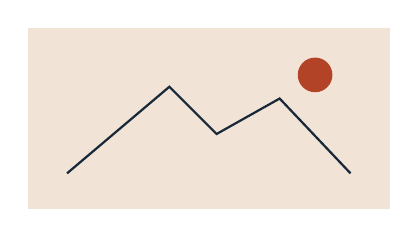
\begin{tikzpicture}[x=1cm,y=1cm]
      \fill[tint] (0,0) rectangle (4.6,2.3);
      \draw[ink,thick] (.5,.45) -- (1.8,1.55) -- (2.4,.95) -- (3.2,1.4) -- (4.1,.45);
      \fill[accent] (3.65,1.7) circle (2.2mm);
    \end{tikzpicture}
  \end{center}
  Replace the drawing with a photo or keep the page all text.
  \PageNo{02}
}
\ZinePage{3}{
  \Kicker{03 / PRINT}
  \Headline{One side only}
  Print the landscape sheet at \textbf{Actual Size (100\%)} on A4, or select US Letter in the source first.
  \medskip\par
  The top row is upside down on purpose.
  \PageNo{03}
}
\ZinePage{4}{
  \Kicker{04 / CREASE}
  \Headline{Make eight panels}
  Crease the sheet once down its length and three times across its width, following the dashed guides.
  \medskip\par
  Unfold it flat before making the cut.
  \PageNo{04}
}
\ZinePage{5}{
  \Kicker{05 / CUT}
  \Headline{Just one slit}
  Cut along the \textbf{solid middle line only}: start at the first vertical fold and stop at the third.
  \medskip\par
  Leave both outer sections attached.
  \PageNo{05}
}
\ZinePage{6}{
  \Kicker{06 / FOLD}
  \Headline{Push the ends in}
  Fold lengthwise with the print facing out. Push the two short ends toward each other until the slit opens into a diamond.
  \medskip\par
  Flatten the diamond into a cross, then wrap the panels until the front and back covers are on the outside.
  \PageNo{06}
}
\ZinePage{7}{
  \Kicker{BACK COVER}
  \vspace{15mm}
  {\sffamily\bfseries\LARGE Made to fold.\par}\medskip
  One sheet of paper.\par
  No staples or glue.\par
  \vspace{7mm}
  {\color{accent}\rule{20mm}{1.3pt}}
}

% ---- Imposition engine. You shouldn't need to edit below this line. ----
\newsavebox\PanelContent
\newcommand\PanelBox[1]{%
  \begin{lrbox}{\PanelContent}%
    \begin{minipage}{\InnerW}%
      \raggedright\normalfont\normalsize\color{ink}%
      \setlength\parskip{3pt}%
      \csname zinepage#1\endcsname\par
    \end{minipage}%
  \end{lrbox}%
  \ifdim\dimexpr\ht\PanelContent+\dp\PanelContent\relax>\InnerH
    \PackageWarningNoLine{mini-zine}{Panel #1 exceeds the safe height; shorten the content}%
  \fi
  \begin{minipage}[c][\InnerH][t]{\InnerW}%
    \noindent\usebox\PanelContent\par
  \end{minipage}%
}
\newcommand\ZineSheet{%
  \null
  \begin{tikzpicture}[remember picture,overlay]
    \begin{scope}[shift={(current page.south west)},x=\PanelW,y=\PanelH]
      % Printed view, left to right: 6 5 4 3 up top; back front 1 2 below.
      \foreach \p [count=\i from 0] in {7,0,1,2}
        \node[inner sep=0pt,outer sep=0pt] at ({\i+.5},.5) {\PanelBox{\p}};
      \foreach \p [count=\i from 0] in {6,5,4,3}
        \node[inner sep=0pt,outer sep=0pt,rotate=180] at ({\i+.5},1.5) {\PanelBox{\p}};
      \ifdefined\ZineNoGuides\else
        \foreach \x in {1,2,3}
          \draw[muted!60,dashed,line width=.3pt] ([yshift=5mm]\x,0) -- ([yshift=-5mm]\x,2);
        \draw[muted!60,dashed,line width=.3pt] ([xshift=5mm]0,1) -- (1,1);
        \draw[muted!60,dashed,line width=.3pt] (3,1) -- ([xshift=-5mm]4,1);
        \draw[accent,line width=.65pt] (1,1) -- (3,1);
      \fi
    \end{scope}
  \end{tikzpicture}%
}
\newcommand\ZineReadPage[1]{%
  \null
  \begin{tikzpicture}[remember picture,overlay]
    \node[inner sep=0pt,outer sep=0pt] at (current page.center) {\PanelBox{#1}};
  \end{tikzpicture}%
}

\begin{document}
\ifdefined\ZinePreview
  \ZineReadPage{0}\newpage\ZineReadPage{1}\newpage
  \ZineReadPage{2}\newpage\ZineReadPage{3}\newpage
  \ZineReadPage{4}\newpage\ZineReadPage{5}\newpage
  \ZineReadPage{6}\newpage\ZineReadPage{7}
\else
  \ZineSheet
\fi
\end{document}
"
% Clean:   pdflatex -jobname=mini-zine-clean "\def\ZineNoGuides{1}% ONE SHEET / EIGHT PAGES — single-file LaTeX mini-zine
% Print:   pdflatex mini-zine.tex  (run twice to resolve page positions)
% Preview: pdflatex -jobname=mini-zine-preview "\def\ZinePreview{1}% ONE SHEET / EIGHT PAGES — single-file LaTeX mini-zine
% Print:   pdflatex mini-zine.tex  (run twice to resolve page positions)
% Preview: pdflatex -jobname=mini-zine-preview "\def\ZinePreview{1}\input{mini-zine.tex}"
% Clean:   pdflatex -jobname=mini-zine-clean "\def\ZineNoGuides{1}\input{mini-zine.tex}"
% US Letter: uncomment \def\ZineLetter{1} below (or define it on the command line).
% Layout reference: https://github.com/krthr/fanzines.app#geometra-e-imposicin
% Print one-sided in landscape at Actual Size (100%), not "Fit".
% Crease the 4 x 2 grid. Cut ONLY the solid center segment between the
% first and third vertical folds. Fold lengthwise, print facing out, then
% push the two ends together; flatten the resulting cross into a booklet.
% \ZinePage{0} is the front, 1--6 are inside, and 7 is the back.
% Images: \includegraphics[width=\linewidth,height=30mm,keepaspectratio]{photo.jpg}

\RequirePackage{fix-cm}
\documentclass[10pt]{article}
\usepackage{geometry}
\usepackage{tikz}
\usepackage{graphicx}

% \def\ZineLetter{1}

\newlength\SheetW \newlength\SheetH
\newlength\PanelW \newlength\PanelH
\newlength\SafeMargin \setlength\SafeMargin{6mm}
\newlength\InnerW \newlength\InnerH
\ifdefined\ZineLetter
  \setlength\SheetW{11in} \setlength\SheetH{8.5in}
\else
  \setlength\SheetW{297mm} \setlength\SheetH{210mm}
\fi
\setlength\PanelW{\dimexpr\SheetW/4\relax}
\setlength\PanelH{\dimexpr\SheetH/2\relax}
\setlength\InnerW{\dimexpr\PanelW-2\SafeMargin\relax}
\setlength\InnerH{\dimexpr\PanelH-2\SafeMargin\relax}
\ifdefined\ZinePreview
  \geometry{paperwidth=\PanelW,paperheight=\PanelH,margin=0pt}
\else
  \geometry{paperwidth=\SheetW,paperheight=\SheetH,margin=0pt}
\fi
\pagestyle{empty}
\setlength\parindent{0pt}

\definecolor{ink}{HTML}{172839}
\definecolor{accent}{HTML}{B34327}
\definecolor{muted}{HTML}{545E6A}
\definecolor{tint}{HTML}{F1E3D6}

% ---- Edit these eight blocks, in reading order. ----
\newcommand\ZinePage[2]{\expandafter\long\expandafter\gdef\csname zinepage#1\endcsname{#2}}
\newcommand\Kicker[1]{\textcolor{accent}{\sffamily\bfseries\scriptsize #1}\par\smallskip}
\newcommand\Headline[1]{{\sffamily\bfseries\LARGE #1\par}\medskip}
\newcommand\PageNo[1]{\par\vspace{6mm}{\color{muted}\sffamily\scriptsize #1\par}}

\ZinePage{0}{
  \Kicker{A ONE-SHEET MINI-ZINE}
  \vspace{7mm}
  {\sffamily\bfseries\fontsize{27}{30}\selectfont
  One sheet.\par Eight pages.\par}
  \vspace{6mm}
  {\color{accent}\rule{20mm}{1.3pt}}\par\medskip
  Write it in order.\par Fold it into a book.
}
\ZinePage{1}{
  \Kicker{01 / WRITE}
  \Headline{Start here}
  Each page lives in a \texttt{\string\ZinePage} block. Write the cover, six inside pages, and the back in reading order.
  \medskip\par
  LaTeX takes care of flipping and rearranging them on the print sheet.
  \PageNo{01}
}
\ZinePage{2}{
  \Kicker{02 / DESIGN}
  \Headline{Make it yours}
  Use normal LaTeX: headings, lists, math, photos, or drawings.
  \begin{center}
    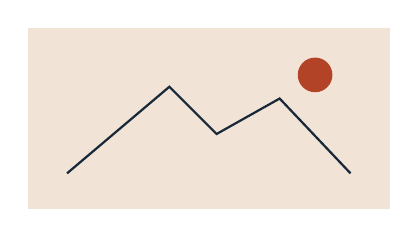
\begin{tikzpicture}[x=1cm,y=1cm]
      \fill[tint] (0,0) rectangle (4.6,2.3);
      \draw[ink,thick] (.5,.45) -- (1.8,1.55) -- (2.4,.95) -- (3.2,1.4) -- (4.1,.45);
      \fill[accent] (3.65,1.7) circle (2.2mm);
    \end{tikzpicture}
  \end{center}
  Replace the drawing with a photo or keep the page all text.
  \PageNo{02}
}
\ZinePage{3}{
  \Kicker{03 / PRINT}
  \Headline{One side only}
  Print the landscape sheet at \textbf{Actual Size (100\%)} on A4, or select US Letter in the source first.
  \medskip\par
  The top row is upside down on purpose.
  \PageNo{03}
}
\ZinePage{4}{
  \Kicker{04 / CREASE}
  \Headline{Make eight panels}
  Crease the sheet once down its length and three times across its width, following the dashed guides.
  \medskip\par
  Unfold it flat before making the cut.
  \PageNo{04}
}
\ZinePage{5}{
  \Kicker{05 / CUT}
  \Headline{Just one slit}
  Cut along the \textbf{solid middle line only}: start at the first vertical fold and stop at the third.
  \medskip\par
  Leave both outer sections attached.
  \PageNo{05}
}
\ZinePage{6}{
  \Kicker{06 / FOLD}
  \Headline{Push the ends in}
  Fold lengthwise with the print facing out. Push the two short ends toward each other until the slit opens into a diamond.
  \medskip\par
  Flatten the diamond into a cross, then wrap the panels until the front and back covers are on the outside.
  \PageNo{06}
}
\ZinePage{7}{
  \Kicker{BACK COVER}
  \vspace{15mm}
  {\sffamily\bfseries\LARGE Made to fold.\par}\medskip
  One sheet of paper.\par
  No staples or glue.\par
  \vspace{7mm}
  {\color{accent}\rule{20mm}{1.3pt}}
}

% ---- Imposition engine. You shouldn't need to edit below this line. ----
\newsavebox\PanelContent
\newcommand\PanelBox[1]{%
  \begin{lrbox}{\PanelContent}%
    \begin{minipage}{\InnerW}%
      \raggedright\normalfont\normalsize\color{ink}%
      \setlength\parskip{3pt}%
      \csname zinepage#1\endcsname\par
    \end{minipage}%
  \end{lrbox}%
  \ifdim\dimexpr\ht\PanelContent+\dp\PanelContent\relax>\InnerH
    \PackageWarningNoLine{mini-zine}{Panel #1 exceeds the safe height; shorten the content}%
  \fi
  \begin{minipage}[c][\InnerH][t]{\InnerW}%
    \noindent\usebox\PanelContent\par
  \end{minipage}%
}
\newcommand\ZineSheet{%
  \null
  \begin{tikzpicture}[remember picture,overlay]
    \begin{scope}[shift={(current page.south west)},x=\PanelW,y=\PanelH]
      % Printed view, left to right: 6 5 4 3 up top; back front 1 2 below.
      \foreach \p [count=\i from 0] in {7,0,1,2}
        \node[inner sep=0pt,outer sep=0pt] at ({\i+.5},.5) {\PanelBox{\p}};
      \foreach \p [count=\i from 0] in {6,5,4,3}
        \node[inner sep=0pt,outer sep=0pt,rotate=180] at ({\i+.5},1.5) {\PanelBox{\p}};
      \ifdefined\ZineNoGuides\else
        \foreach \x in {1,2,3}
          \draw[muted!60,dashed,line width=.3pt] ([yshift=5mm]\x,0) -- ([yshift=-5mm]\x,2);
        \draw[muted!60,dashed,line width=.3pt] ([xshift=5mm]0,1) -- (1,1);
        \draw[muted!60,dashed,line width=.3pt] (3,1) -- ([xshift=-5mm]4,1);
        \draw[accent,line width=.65pt] (1,1) -- (3,1);
      \fi
    \end{scope}
  \end{tikzpicture}%
}
\newcommand\ZineReadPage[1]{%
  \null
  \begin{tikzpicture}[remember picture,overlay]
    \node[inner sep=0pt,outer sep=0pt] at (current page.center) {\PanelBox{#1}};
  \end{tikzpicture}%
}

\begin{document}
\ifdefined\ZinePreview
  \ZineReadPage{0}\newpage\ZineReadPage{1}\newpage
  \ZineReadPage{2}\newpage\ZineReadPage{3}\newpage
  \ZineReadPage{4}\newpage\ZineReadPage{5}\newpage
  \ZineReadPage{6}\newpage\ZineReadPage{7}
\else
  \ZineSheet
\fi
\end{document}
"
% Clean:   pdflatex -jobname=mini-zine-clean "\def\ZineNoGuides{1}% ONE SHEET / EIGHT PAGES — single-file LaTeX mini-zine
% Print:   pdflatex mini-zine.tex  (run twice to resolve page positions)
% Preview: pdflatex -jobname=mini-zine-preview "\def\ZinePreview{1}\input{mini-zine.tex}"
% Clean:   pdflatex -jobname=mini-zine-clean "\def\ZineNoGuides{1}\input{mini-zine.tex}"
% US Letter: uncomment \def\ZineLetter{1} below (or define it on the command line).
% Layout reference: https://github.com/krthr/fanzines.app#geometra-e-imposicin
% Print one-sided in landscape at Actual Size (100%), not "Fit".
% Crease the 4 x 2 grid. Cut ONLY the solid center segment between the
% first and third vertical folds. Fold lengthwise, print facing out, then
% push the two ends together; flatten the resulting cross into a booklet.
% \ZinePage{0} is the front, 1--6 are inside, and 7 is the back.
% Images: \includegraphics[width=\linewidth,height=30mm,keepaspectratio]{photo.jpg}

\RequirePackage{fix-cm}
\documentclass[10pt]{article}
\usepackage{geometry}
\usepackage{tikz}
\usepackage{graphicx}

% \def\ZineLetter{1}

\newlength\SheetW \newlength\SheetH
\newlength\PanelW \newlength\PanelH
\newlength\SafeMargin \setlength\SafeMargin{6mm}
\newlength\InnerW \newlength\InnerH
\ifdefined\ZineLetter
  \setlength\SheetW{11in} \setlength\SheetH{8.5in}
\else
  \setlength\SheetW{297mm} \setlength\SheetH{210mm}
\fi
\setlength\PanelW{\dimexpr\SheetW/4\relax}
\setlength\PanelH{\dimexpr\SheetH/2\relax}
\setlength\InnerW{\dimexpr\PanelW-2\SafeMargin\relax}
\setlength\InnerH{\dimexpr\PanelH-2\SafeMargin\relax}
\ifdefined\ZinePreview
  \geometry{paperwidth=\PanelW,paperheight=\PanelH,margin=0pt}
\else
  \geometry{paperwidth=\SheetW,paperheight=\SheetH,margin=0pt}
\fi
\pagestyle{empty}
\setlength\parindent{0pt}

\definecolor{ink}{HTML}{172839}
\definecolor{accent}{HTML}{B34327}
\definecolor{muted}{HTML}{545E6A}
\definecolor{tint}{HTML}{F1E3D6}

% ---- Edit these eight blocks, in reading order. ----
\newcommand\ZinePage[2]{\expandafter\long\expandafter\gdef\csname zinepage#1\endcsname{#2}}
\newcommand\Kicker[1]{\textcolor{accent}{\sffamily\bfseries\scriptsize #1}\par\smallskip}
\newcommand\Headline[1]{{\sffamily\bfseries\LARGE #1\par}\medskip}
\newcommand\PageNo[1]{\par\vspace{6mm}{\color{muted}\sffamily\scriptsize #1\par}}

\ZinePage{0}{
  \Kicker{A ONE-SHEET MINI-ZINE}
  \vspace{7mm}
  {\sffamily\bfseries\fontsize{27}{30}\selectfont
  One sheet.\par Eight pages.\par}
  \vspace{6mm}
  {\color{accent}\rule{20mm}{1.3pt}}\par\medskip
  Write it in order.\par Fold it into a book.
}
\ZinePage{1}{
  \Kicker{01 / WRITE}
  \Headline{Start here}
  Each page lives in a \texttt{\string\ZinePage} block. Write the cover, six inside pages, and the back in reading order.
  \medskip\par
  LaTeX takes care of flipping and rearranging them on the print sheet.
  \PageNo{01}
}
\ZinePage{2}{
  \Kicker{02 / DESIGN}
  \Headline{Make it yours}
  Use normal LaTeX: headings, lists, math, photos, or drawings.
  \begin{center}
    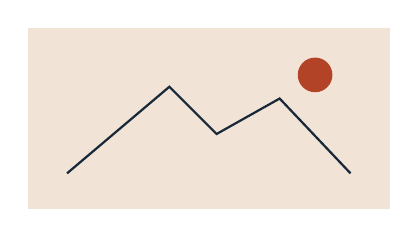
\begin{tikzpicture}[x=1cm,y=1cm]
      \fill[tint] (0,0) rectangle (4.6,2.3);
      \draw[ink,thick] (.5,.45) -- (1.8,1.55) -- (2.4,.95) -- (3.2,1.4) -- (4.1,.45);
      \fill[accent] (3.65,1.7) circle (2.2mm);
    \end{tikzpicture}
  \end{center}
  Replace the drawing with a photo or keep the page all text.
  \PageNo{02}
}
\ZinePage{3}{
  \Kicker{03 / PRINT}
  \Headline{One side only}
  Print the landscape sheet at \textbf{Actual Size (100\%)} on A4, or select US Letter in the source first.
  \medskip\par
  The top row is upside down on purpose.
  \PageNo{03}
}
\ZinePage{4}{
  \Kicker{04 / CREASE}
  \Headline{Make eight panels}
  Crease the sheet once down its length and three times across its width, following the dashed guides.
  \medskip\par
  Unfold it flat before making the cut.
  \PageNo{04}
}
\ZinePage{5}{
  \Kicker{05 / CUT}
  \Headline{Just one slit}
  Cut along the \textbf{solid middle line only}: start at the first vertical fold and stop at the third.
  \medskip\par
  Leave both outer sections attached.
  \PageNo{05}
}
\ZinePage{6}{
  \Kicker{06 / FOLD}
  \Headline{Push the ends in}
  Fold lengthwise with the print facing out. Push the two short ends toward each other until the slit opens into a diamond.
  \medskip\par
  Flatten the diamond into a cross, then wrap the panels until the front and back covers are on the outside.
  \PageNo{06}
}
\ZinePage{7}{
  \Kicker{BACK COVER}
  \vspace{15mm}
  {\sffamily\bfseries\LARGE Made to fold.\par}\medskip
  One sheet of paper.\par
  No staples or glue.\par
  \vspace{7mm}
  {\color{accent}\rule{20mm}{1.3pt}}
}

% ---- Imposition engine. You shouldn't need to edit below this line. ----
\newsavebox\PanelContent
\newcommand\PanelBox[1]{%
  \begin{lrbox}{\PanelContent}%
    \begin{minipage}{\InnerW}%
      \raggedright\normalfont\normalsize\color{ink}%
      \setlength\parskip{3pt}%
      \csname zinepage#1\endcsname\par
    \end{minipage}%
  \end{lrbox}%
  \ifdim\dimexpr\ht\PanelContent+\dp\PanelContent\relax>\InnerH
    \PackageWarningNoLine{mini-zine}{Panel #1 exceeds the safe height; shorten the content}%
  \fi
  \begin{minipage}[c][\InnerH][t]{\InnerW}%
    \noindent\usebox\PanelContent\par
  \end{minipage}%
}
\newcommand\ZineSheet{%
  \null
  \begin{tikzpicture}[remember picture,overlay]
    \begin{scope}[shift={(current page.south west)},x=\PanelW,y=\PanelH]
      % Printed view, left to right: 6 5 4 3 up top; back front 1 2 below.
      \foreach \p [count=\i from 0] in {7,0,1,2}
        \node[inner sep=0pt,outer sep=0pt] at ({\i+.5},.5) {\PanelBox{\p}};
      \foreach \p [count=\i from 0] in {6,5,4,3}
        \node[inner sep=0pt,outer sep=0pt,rotate=180] at ({\i+.5},1.5) {\PanelBox{\p}};
      \ifdefined\ZineNoGuides\else
        \foreach \x in {1,2,3}
          \draw[muted!60,dashed,line width=.3pt] ([yshift=5mm]\x,0) -- ([yshift=-5mm]\x,2);
        \draw[muted!60,dashed,line width=.3pt] ([xshift=5mm]0,1) -- (1,1);
        \draw[muted!60,dashed,line width=.3pt] (3,1) -- ([xshift=-5mm]4,1);
        \draw[accent,line width=.65pt] (1,1) -- (3,1);
      \fi
    \end{scope}
  \end{tikzpicture}%
}
\newcommand\ZineReadPage[1]{%
  \null
  \begin{tikzpicture}[remember picture,overlay]
    \node[inner sep=0pt,outer sep=0pt] at (current page.center) {\PanelBox{#1}};
  \end{tikzpicture}%
}

\begin{document}
\ifdefined\ZinePreview
  \ZineReadPage{0}\newpage\ZineReadPage{1}\newpage
  \ZineReadPage{2}\newpage\ZineReadPage{3}\newpage
  \ZineReadPage{4}\newpage\ZineReadPage{5}\newpage
  \ZineReadPage{6}\newpage\ZineReadPage{7}
\else
  \ZineSheet
\fi
\end{document}
"
% US Letter: uncomment \def\ZineLetter{1} below (or define it on the command line).
% Layout reference: https://github.com/krthr/fanzines.app#geometra-e-imposicin
% Print one-sided in landscape at Actual Size (100%), not "Fit".
% Crease the 4 x 2 grid. Cut ONLY the solid center segment between the
% first and third vertical folds. Fold lengthwise, print facing out, then
% push the two ends together; flatten the resulting cross into a booklet.
% \ZinePage{0} is the front, 1--6 are inside, and 7 is the back.
% Images: \includegraphics[width=\linewidth,height=30mm,keepaspectratio]{photo.jpg}

\RequirePackage{fix-cm}
\documentclass[10pt]{article}
\usepackage{geometry}
\usepackage{tikz}
\usepackage{graphicx}

% \def\ZineLetter{1}

\newlength\SheetW \newlength\SheetH
\newlength\PanelW \newlength\PanelH
\newlength\SafeMargin \setlength\SafeMargin{6mm}
\newlength\InnerW \newlength\InnerH
\ifdefined\ZineLetter
  \setlength\SheetW{11in} \setlength\SheetH{8.5in}
\else
  \setlength\SheetW{297mm} \setlength\SheetH{210mm}
\fi
\setlength\PanelW{\dimexpr\SheetW/4\relax}
\setlength\PanelH{\dimexpr\SheetH/2\relax}
\setlength\InnerW{\dimexpr\PanelW-2\SafeMargin\relax}
\setlength\InnerH{\dimexpr\PanelH-2\SafeMargin\relax}
\ifdefined\ZinePreview
  \geometry{paperwidth=\PanelW,paperheight=\PanelH,margin=0pt}
\else
  \geometry{paperwidth=\SheetW,paperheight=\SheetH,margin=0pt}
\fi
\pagestyle{empty}
\setlength\parindent{0pt}

\definecolor{ink}{HTML}{172839}
\definecolor{accent}{HTML}{B34327}
\definecolor{muted}{HTML}{545E6A}
\definecolor{tint}{HTML}{F1E3D6}

% ---- Edit these eight blocks, in reading order. ----
\newcommand\ZinePage[2]{\expandafter\long\expandafter\gdef\csname zinepage#1\endcsname{#2}}
\newcommand\Kicker[1]{\textcolor{accent}{\sffamily\bfseries\scriptsize #1}\par\smallskip}
\newcommand\Headline[1]{{\sffamily\bfseries\LARGE #1\par}\medskip}
\newcommand\PageNo[1]{\par\vspace{6mm}{\color{muted}\sffamily\scriptsize #1\par}}

\ZinePage{0}{
  \Kicker{A ONE-SHEET MINI-ZINE}
  \vspace{7mm}
  {\sffamily\bfseries\fontsize{27}{30}\selectfont
  One sheet.\par Eight pages.\par}
  \vspace{6mm}
  {\color{accent}\rule{20mm}{1.3pt}}\par\medskip
  Write it in order.\par Fold it into a book.
}
\ZinePage{1}{
  \Kicker{01 / WRITE}
  \Headline{Start here}
  Each page lives in a \texttt{\string\ZinePage} block. Write the cover, six inside pages, and the back in reading order.
  \medskip\par
  LaTeX takes care of flipping and rearranging them on the print sheet.
  \PageNo{01}
}
\ZinePage{2}{
  \Kicker{02 / DESIGN}
  \Headline{Make it yours}
  Use normal LaTeX: headings, lists, math, photos, or drawings.
  \begin{center}
    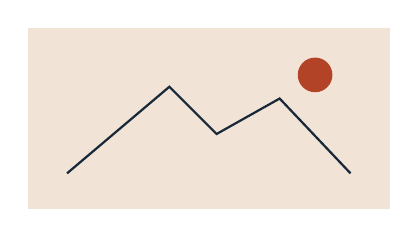
\begin{tikzpicture}[x=1cm,y=1cm]
      \fill[tint] (0,0) rectangle (4.6,2.3);
      \draw[ink,thick] (.5,.45) -- (1.8,1.55) -- (2.4,.95) -- (3.2,1.4) -- (4.1,.45);
      \fill[accent] (3.65,1.7) circle (2.2mm);
    \end{tikzpicture}
  \end{center}
  Replace the drawing with a photo or keep the page all text.
  \PageNo{02}
}
\ZinePage{3}{
  \Kicker{03 / PRINT}
  \Headline{One side only}
  Print the landscape sheet at \textbf{Actual Size (100\%)} on A4, or select US Letter in the source first.
  \medskip\par
  The top row is upside down on purpose.
  \PageNo{03}
}
\ZinePage{4}{
  \Kicker{04 / CREASE}
  \Headline{Make eight panels}
  Crease the sheet once down its length and three times across its width, following the dashed guides.
  \medskip\par
  Unfold it flat before making the cut.
  \PageNo{04}
}
\ZinePage{5}{
  \Kicker{05 / CUT}
  \Headline{Just one slit}
  Cut along the \textbf{solid middle line only}: start at the first vertical fold and stop at the third.
  \medskip\par
  Leave both outer sections attached.
  \PageNo{05}
}
\ZinePage{6}{
  \Kicker{06 / FOLD}
  \Headline{Push the ends in}
  Fold lengthwise with the print facing out. Push the two short ends toward each other until the slit opens into a diamond.
  \medskip\par
  Flatten the diamond into a cross, then wrap the panels until the front and back covers are on the outside.
  \PageNo{06}
}
\ZinePage{7}{
  \Kicker{BACK COVER}
  \vspace{15mm}
  {\sffamily\bfseries\LARGE Made to fold.\par}\medskip
  One sheet of paper.\par
  No staples or glue.\par
  \vspace{7mm}
  {\color{accent}\rule{20mm}{1.3pt}}
}

% ---- Imposition engine. You shouldn't need to edit below this line. ----
\newsavebox\PanelContent
\newcommand\PanelBox[1]{%
  \begin{lrbox}{\PanelContent}%
    \begin{minipage}{\InnerW}%
      \raggedright\normalfont\normalsize\color{ink}%
      \setlength\parskip{3pt}%
      \csname zinepage#1\endcsname\par
    \end{minipage}%
  \end{lrbox}%
  \ifdim\dimexpr\ht\PanelContent+\dp\PanelContent\relax>\InnerH
    \PackageWarningNoLine{mini-zine}{Panel #1 exceeds the safe height; shorten the content}%
  \fi
  \begin{minipage}[c][\InnerH][t]{\InnerW}%
    \noindent\usebox\PanelContent\par
  \end{minipage}%
}
\newcommand\ZineSheet{%
  \null
  \begin{tikzpicture}[remember picture,overlay]
    \begin{scope}[shift={(current page.south west)},x=\PanelW,y=\PanelH]
      % Printed view, left to right: 6 5 4 3 up top; back front 1 2 below.
      \foreach \p [count=\i from 0] in {7,0,1,2}
        \node[inner sep=0pt,outer sep=0pt] at ({\i+.5},.5) {\PanelBox{\p}};
      \foreach \p [count=\i from 0] in {6,5,4,3}
        \node[inner sep=0pt,outer sep=0pt,rotate=180] at ({\i+.5},1.5) {\PanelBox{\p}};
      \ifdefined\ZineNoGuides\else
        \foreach \x in {1,2,3}
          \draw[muted!60,dashed,line width=.3pt] ([yshift=5mm]\x,0) -- ([yshift=-5mm]\x,2);
        \draw[muted!60,dashed,line width=.3pt] ([xshift=5mm]0,1) -- (1,1);
        \draw[muted!60,dashed,line width=.3pt] (3,1) -- ([xshift=-5mm]4,1);
        \draw[accent,line width=.65pt] (1,1) -- (3,1);
      \fi
    \end{scope}
  \end{tikzpicture}%
}
\newcommand\ZineReadPage[1]{%
  \null
  \begin{tikzpicture}[remember picture,overlay]
    \node[inner sep=0pt,outer sep=0pt] at (current page.center) {\PanelBox{#1}};
  \end{tikzpicture}%
}

\begin{document}
\ifdefined\ZinePreview
  \ZineReadPage{0}\newpage\ZineReadPage{1}\newpage
  \ZineReadPage{2}\newpage\ZineReadPage{3}\newpage
  \ZineReadPage{4}\newpage\ZineReadPage{5}\newpage
  \ZineReadPage{6}\newpage\ZineReadPage{7}
\else
  \ZineSheet
\fi
\end{document}
"
% US Letter: uncomment \def\ZineLetter{1} below (or define it on the command line).
% Layout reference: https://github.com/krthr/fanzines.app#geometra-e-imposicin
% Print one-sided in landscape at Actual Size (100%), not "Fit".
% Crease the 4 x 2 grid. Cut ONLY the solid center segment between the
% first and third vertical folds. Fold lengthwise, print facing out, then
% push the two ends together; flatten the resulting cross into a booklet.
% \ZinePage{0} is the front, 1--6 are inside, and 7 is the back.
% Images: \includegraphics[width=\linewidth,height=30mm,keepaspectratio]{photo.jpg}

\RequirePackage{fix-cm}
\documentclass[10pt]{article}
\usepackage{geometry}
\usepackage{tikz}
\usepackage{graphicx}

% \def\ZineLetter{1}

\newlength\SheetW \newlength\SheetH
\newlength\PanelW \newlength\PanelH
\newlength\SafeMargin \setlength\SafeMargin{6mm}
\newlength\InnerW \newlength\InnerH
\ifdefined\ZineLetter
  \setlength\SheetW{11in} \setlength\SheetH{8.5in}
\else
  \setlength\SheetW{297mm} \setlength\SheetH{210mm}
\fi
\setlength\PanelW{\dimexpr\SheetW/4\relax}
\setlength\PanelH{\dimexpr\SheetH/2\relax}
\setlength\InnerW{\dimexpr\PanelW-2\SafeMargin\relax}
\setlength\InnerH{\dimexpr\PanelH-2\SafeMargin\relax}
\ifdefined\ZinePreview
  \geometry{paperwidth=\PanelW,paperheight=\PanelH,margin=0pt}
\else
  \geometry{paperwidth=\SheetW,paperheight=\SheetH,margin=0pt}
\fi
\pagestyle{empty}
\setlength\parindent{0pt}

\definecolor{ink}{HTML}{172839}
\definecolor{accent}{HTML}{B34327}
\definecolor{muted}{HTML}{545E6A}
\definecolor{tint}{HTML}{F1E3D6}

% ---- Edit these eight blocks, in reading order. ----
\newcommand\ZinePage[2]{\expandafter\long\expandafter\gdef\csname zinepage#1\endcsname{#2}}
\newcommand\Kicker[1]{\textcolor{accent}{\sffamily\bfseries\scriptsize #1}\par\smallskip}
\newcommand\Headline[1]{{\sffamily\bfseries\LARGE #1\par}\medskip}
\newcommand\PageNo[1]{\par\vspace{6mm}{\color{muted}\sffamily\scriptsize #1\par}}

\ZinePage{0}{
  \Kicker{A ONE-SHEET MINI-ZINE}
  \vspace{7mm}
  {\sffamily\bfseries\fontsize{27}{30}\selectfont
  One sheet.\par Eight pages.\par}
  \vspace{6mm}
  {\color{accent}\rule{20mm}{1.3pt}}\par\medskip
  Write it in order.\par Fold it into a book.
}
\ZinePage{1}{
  \Kicker{01 / WRITE}
  \Headline{Start here}
  Each page lives in a \texttt{\string\ZinePage} block. Write the cover, six inside pages, and the back in reading order.
  \medskip\par
  LaTeX takes care of flipping and rearranging them on the print sheet.
  \PageNo{01}
}
\ZinePage{2}{
  \Kicker{02 / DESIGN}
  \Headline{Make it yours}
  Use normal LaTeX: headings, lists, math, photos, or drawings.
  \begin{center}
    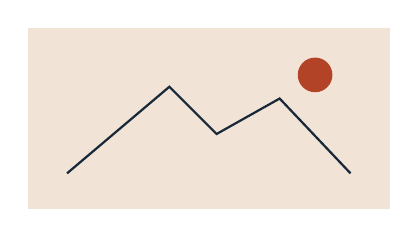
\begin{tikzpicture}[x=1cm,y=1cm]
      \fill[tint] (0,0) rectangle (4.6,2.3);
      \draw[ink,thick] (.5,.45) -- (1.8,1.55) -- (2.4,.95) -- (3.2,1.4) -- (4.1,.45);
      \fill[accent] (3.65,1.7) circle (2.2mm);
    \end{tikzpicture}
  \end{center}
  Replace the drawing with a photo or keep the page all text.
  \PageNo{02}
}
\ZinePage{3}{
  \Kicker{03 / PRINT}
  \Headline{One side only}
  Print the landscape sheet at \textbf{Actual Size (100\%)} on A4, or select US Letter in the source first.
  \medskip\par
  The top row is upside down on purpose.
  \PageNo{03}
}
\ZinePage{4}{
  \Kicker{04 / CREASE}
  \Headline{Make eight panels}
  Crease the sheet once down its length and three times across its width, following the dashed guides.
  \medskip\par
  Unfold it flat before making the cut.
  \PageNo{04}
}
\ZinePage{5}{
  \Kicker{05 / CUT}
  \Headline{Just one slit}
  Cut along the \textbf{solid middle line only}: start at the first vertical fold and stop at the third.
  \medskip\par
  Leave both outer sections attached.
  \PageNo{05}
}
\ZinePage{6}{
  \Kicker{06 / FOLD}
  \Headline{Push the ends in}
  Fold lengthwise with the print facing out. Push the two short ends toward each other until the slit opens into a diamond.
  \medskip\par
  Flatten the diamond into a cross, then wrap the panels until the front and back covers are on the outside.
  \PageNo{06}
}
\ZinePage{7}{
  \Kicker{BACK COVER}
  \vspace{15mm}
  {\sffamily\bfseries\LARGE Made to fold.\par}\medskip
  One sheet of paper.\par
  No staples or glue.\par
  \vspace{7mm}
  {\color{accent}\rule{20mm}{1.3pt}}
}

% ---- Imposition engine. You shouldn't need to edit below this line. ----
\newsavebox\PanelContent
\newcommand\PanelBox[1]{%
  \begin{lrbox}{\PanelContent}%
    \begin{minipage}{\InnerW}%
      \raggedright\normalfont\normalsize\color{ink}%
      \setlength\parskip{3pt}%
      \csname zinepage#1\endcsname\par
    \end{minipage}%
  \end{lrbox}%
  \ifdim\dimexpr\ht\PanelContent+\dp\PanelContent\relax>\InnerH
    \PackageWarningNoLine{mini-zine}{Panel #1 exceeds the safe height; shorten the content}%
  \fi
  \begin{minipage}[c][\InnerH][t]{\InnerW}%
    \noindent\usebox\PanelContent\par
  \end{minipage}%
}
\newcommand\ZineSheet{%
  \null
  \begin{tikzpicture}[remember picture,overlay]
    \begin{scope}[shift={(current page.south west)},x=\PanelW,y=\PanelH]
      % Printed view, left to right: 6 5 4 3 up top; back front 1 2 below.
      \foreach \p [count=\i from 0] in {7,0,1,2}
        \node[inner sep=0pt,outer sep=0pt] at ({\i+.5},.5) {\PanelBox{\p}};
      \foreach \p [count=\i from 0] in {6,5,4,3}
        \node[inner sep=0pt,outer sep=0pt,rotate=180] at ({\i+.5},1.5) {\PanelBox{\p}};
      \ifdefined\ZineNoGuides\else
        \foreach \x in {1,2,3}
          \draw[muted!60,dashed,line width=.3pt] ([yshift=5mm]\x,0) -- ([yshift=-5mm]\x,2);
        \draw[muted!60,dashed,line width=.3pt] ([xshift=5mm]0,1) -- (1,1);
        \draw[muted!60,dashed,line width=.3pt] (3,1) -- ([xshift=-5mm]4,1);
        \draw[accent,line width=.65pt] (1,1) -- (3,1);
      \fi
    \end{scope}
  \end{tikzpicture}%
}
\newcommand\ZineReadPage[1]{%
  \null
  \begin{tikzpicture}[remember picture,overlay]
    \node[inner sep=0pt,outer sep=0pt] at (current page.center) {\PanelBox{#1}};
  \end{tikzpicture}%
}

\begin{document}
\ifdefined\ZinePreview
  \ZineReadPage{0}\newpage\ZineReadPage{1}\newpage
  \ZineReadPage{2}\newpage\ZineReadPage{3}\newpage
  \ZineReadPage{4}\newpage\ZineReadPage{5}\newpage
  \ZineReadPage{6}\newpage\ZineReadPage{7}
\else
  \ZineSheet
\fi
\end{document}
"
% Clean:   pdflatex -jobname=mini-zine-clean "\def\ZineNoGuides{1}% ONE SHEET / EIGHT PAGES — single-file LaTeX mini-zine
% Print:   pdflatex mini-zine.tex  (run twice to resolve page positions)
% Preview: pdflatex -jobname=mini-zine-preview "\def\ZinePreview{1}% ONE SHEET / EIGHT PAGES — single-file LaTeX mini-zine
% Print:   pdflatex mini-zine.tex  (run twice to resolve page positions)
% Preview: pdflatex -jobname=mini-zine-preview "\def\ZinePreview{1}% ONE SHEET / EIGHT PAGES — single-file LaTeX mini-zine
% Print:   pdflatex mini-zine.tex  (run twice to resolve page positions)
% Preview: pdflatex -jobname=mini-zine-preview "\def\ZinePreview{1}\input{mini-zine.tex}"
% Clean:   pdflatex -jobname=mini-zine-clean "\def\ZineNoGuides{1}\input{mini-zine.tex}"
% US Letter: uncomment \def\ZineLetter{1} below (or define it on the command line).
% Layout reference: https://github.com/krthr/fanzines.app#geometra-e-imposicin
% Print one-sided in landscape at Actual Size (100%), not "Fit".
% Crease the 4 x 2 grid. Cut ONLY the solid center segment between the
% first and third vertical folds. Fold lengthwise, print facing out, then
% push the two ends together; flatten the resulting cross into a booklet.
% \ZinePage{0} is the front, 1--6 are inside, and 7 is the back.
% Images: \includegraphics[width=\linewidth,height=30mm,keepaspectratio]{photo.jpg}

\RequirePackage{fix-cm}
\documentclass[10pt]{article}
\usepackage{geometry}
\usepackage{tikz}
\usepackage{graphicx}

% \def\ZineLetter{1}

\newlength\SheetW \newlength\SheetH
\newlength\PanelW \newlength\PanelH
\newlength\SafeMargin \setlength\SafeMargin{6mm}
\newlength\InnerW \newlength\InnerH
\ifdefined\ZineLetter
  \setlength\SheetW{11in} \setlength\SheetH{8.5in}
\else
  \setlength\SheetW{297mm} \setlength\SheetH{210mm}
\fi
\setlength\PanelW{\dimexpr\SheetW/4\relax}
\setlength\PanelH{\dimexpr\SheetH/2\relax}
\setlength\InnerW{\dimexpr\PanelW-2\SafeMargin\relax}
\setlength\InnerH{\dimexpr\PanelH-2\SafeMargin\relax}
\ifdefined\ZinePreview
  \geometry{paperwidth=\PanelW,paperheight=\PanelH,margin=0pt}
\else
  \geometry{paperwidth=\SheetW,paperheight=\SheetH,margin=0pt}
\fi
\pagestyle{empty}
\setlength\parindent{0pt}

\definecolor{ink}{HTML}{172839}
\definecolor{accent}{HTML}{B34327}
\definecolor{muted}{HTML}{545E6A}
\definecolor{tint}{HTML}{F1E3D6}

% ---- Edit these eight blocks, in reading order. ----
\newcommand\ZinePage[2]{\expandafter\long\expandafter\gdef\csname zinepage#1\endcsname{#2}}
\newcommand\Kicker[1]{\textcolor{accent}{\sffamily\bfseries\scriptsize #1}\par\smallskip}
\newcommand\Headline[1]{{\sffamily\bfseries\LARGE #1\par}\medskip}
\newcommand\PageNo[1]{\par\vspace{6mm}{\color{muted}\sffamily\scriptsize #1\par}}

\ZinePage{0}{
  \Kicker{A ONE-SHEET MINI-ZINE}
  \vspace{7mm}
  {\sffamily\bfseries\fontsize{27}{30}\selectfont
  One sheet.\par Eight pages.\par}
  \vspace{6mm}
  {\color{accent}\rule{20mm}{1.3pt}}\par\medskip
  Write it in order.\par Fold it into a book.
}
\ZinePage{1}{
  \Kicker{01 / WRITE}
  \Headline{Start here}
  Each page lives in a \texttt{\string\ZinePage} block. Write the cover, six inside pages, and the back in reading order.
  \medskip\par
  LaTeX takes care of flipping and rearranging them on the print sheet.
  \PageNo{01}
}
\ZinePage{2}{
  \Kicker{02 / DESIGN}
  \Headline{Make it yours}
  Use normal LaTeX: headings, lists, math, photos, or drawings.
  \begin{center}
    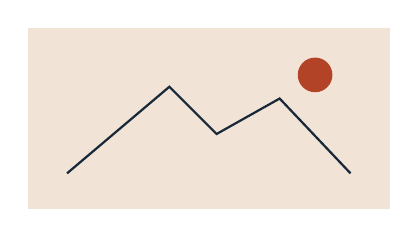
\begin{tikzpicture}[x=1cm,y=1cm]
      \fill[tint] (0,0) rectangle (4.6,2.3);
      \draw[ink,thick] (.5,.45) -- (1.8,1.55) -- (2.4,.95) -- (3.2,1.4) -- (4.1,.45);
      \fill[accent] (3.65,1.7) circle (2.2mm);
    \end{tikzpicture}
  \end{center}
  Replace the drawing with a photo or keep the page all text.
  \PageNo{02}
}
\ZinePage{3}{
  \Kicker{03 / PRINT}
  \Headline{One side only}
  Print the landscape sheet at \textbf{Actual Size (100\%)} on A4, or select US Letter in the source first.
  \medskip\par
  The top row is upside down on purpose.
  \PageNo{03}
}
\ZinePage{4}{
  \Kicker{04 / CREASE}
  \Headline{Make eight panels}
  Crease the sheet once down its length and three times across its width, following the dashed guides.
  \medskip\par
  Unfold it flat before making the cut.
  \PageNo{04}
}
\ZinePage{5}{
  \Kicker{05 / CUT}
  \Headline{Just one slit}
  Cut along the \textbf{solid middle line only}: start at the first vertical fold and stop at the third.
  \medskip\par
  Leave both outer sections attached.
  \PageNo{05}
}
\ZinePage{6}{
  \Kicker{06 / FOLD}
  \Headline{Push the ends in}
  Fold lengthwise with the print facing out. Push the two short ends toward each other until the slit opens into a diamond.
  \medskip\par
  Flatten the diamond into a cross, then wrap the panels until the front and back covers are on the outside.
  \PageNo{06}
}
\ZinePage{7}{
  \Kicker{BACK COVER}
  \vspace{15mm}
  {\sffamily\bfseries\LARGE Made to fold.\par}\medskip
  One sheet of paper.\par
  No staples or glue.\par
  \vspace{7mm}
  {\color{accent}\rule{20mm}{1.3pt}}
}

% ---- Imposition engine. You shouldn't need to edit below this line. ----
\newsavebox\PanelContent
\newcommand\PanelBox[1]{%
  \begin{lrbox}{\PanelContent}%
    \begin{minipage}{\InnerW}%
      \raggedright\normalfont\normalsize\color{ink}%
      \setlength\parskip{3pt}%
      \csname zinepage#1\endcsname\par
    \end{minipage}%
  \end{lrbox}%
  \ifdim\dimexpr\ht\PanelContent+\dp\PanelContent\relax>\InnerH
    \PackageWarningNoLine{mini-zine}{Panel #1 exceeds the safe height; shorten the content}%
  \fi
  \begin{minipage}[c][\InnerH][t]{\InnerW}%
    \noindent\usebox\PanelContent\par
  \end{minipage}%
}
\newcommand\ZineSheet{%
  \null
  \begin{tikzpicture}[remember picture,overlay]
    \begin{scope}[shift={(current page.south west)},x=\PanelW,y=\PanelH]
      % Printed view, left to right: 6 5 4 3 up top; back front 1 2 below.
      \foreach \p [count=\i from 0] in {7,0,1,2}
        \node[inner sep=0pt,outer sep=0pt] at ({\i+.5},.5) {\PanelBox{\p}};
      \foreach \p [count=\i from 0] in {6,5,4,3}
        \node[inner sep=0pt,outer sep=0pt,rotate=180] at ({\i+.5},1.5) {\PanelBox{\p}};
      \ifdefined\ZineNoGuides\else
        \foreach \x in {1,2,3}
          \draw[muted!60,dashed,line width=.3pt] ([yshift=5mm]\x,0) -- ([yshift=-5mm]\x,2);
        \draw[muted!60,dashed,line width=.3pt] ([xshift=5mm]0,1) -- (1,1);
        \draw[muted!60,dashed,line width=.3pt] (3,1) -- ([xshift=-5mm]4,1);
        \draw[accent,line width=.65pt] (1,1) -- (3,1);
      \fi
    \end{scope}
  \end{tikzpicture}%
}
\newcommand\ZineReadPage[1]{%
  \null
  \begin{tikzpicture}[remember picture,overlay]
    \node[inner sep=0pt,outer sep=0pt] at (current page.center) {\PanelBox{#1}};
  \end{tikzpicture}%
}

\begin{document}
\ifdefined\ZinePreview
  \ZineReadPage{0}\newpage\ZineReadPage{1}\newpage
  \ZineReadPage{2}\newpage\ZineReadPage{3}\newpage
  \ZineReadPage{4}\newpage\ZineReadPage{5}\newpage
  \ZineReadPage{6}\newpage\ZineReadPage{7}
\else
  \ZineSheet
\fi
\end{document}
"
% Clean:   pdflatex -jobname=mini-zine-clean "\def\ZineNoGuides{1}% ONE SHEET / EIGHT PAGES — single-file LaTeX mini-zine
% Print:   pdflatex mini-zine.tex  (run twice to resolve page positions)
% Preview: pdflatex -jobname=mini-zine-preview "\def\ZinePreview{1}\input{mini-zine.tex}"
% Clean:   pdflatex -jobname=mini-zine-clean "\def\ZineNoGuides{1}\input{mini-zine.tex}"
% US Letter: uncomment \def\ZineLetter{1} below (or define it on the command line).
% Layout reference: https://github.com/krthr/fanzines.app#geometra-e-imposicin
% Print one-sided in landscape at Actual Size (100%), not "Fit".
% Crease the 4 x 2 grid. Cut ONLY the solid center segment between the
% first and third vertical folds. Fold lengthwise, print facing out, then
% push the two ends together; flatten the resulting cross into a booklet.
% \ZinePage{0} is the front, 1--6 are inside, and 7 is the back.
% Images: \includegraphics[width=\linewidth,height=30mm,keepaspectratio]{photo.jpg}

\RequirePackage{fix-cm}
\documentclass[10pt]{article}
\usepackage{geometry}
\usepackage{tikz}
\usepackage{graphicx}

% \def\ZineLetter{1}

\newlength\SheetW \newlength\SheetH
\newlength\PanelW \newlength\PanelH
\newlength\SafeMargin \setlength\SafeMargin{6mm}
\newlength\InnerW \newlength\InnerH
\ifdefined\ZineLetter
  \setlength\SheetW{11in} \setlength\SheetH{8.5in}
\else
  \setlength\SheetW{297mm} \setlength\SheetH{210mm}
\fi
\setlength\PanelW{\dimexpr\SheetW/4\relax}
\setlength\PanelH{\dimexpr\SheetH/2\relax}
\setlength\InnerW{\dimexpr\PanelW-2\SafeMargin\relax}
\setlength\InnerH{\dimexpr\PanelH-2\SafeMargin\relax}
\ifdefined\ZinePreview
  \geometry{paperwidth=\PanelW,paperheight=\PanelH,margin=0pt}
\else
  \geometry{paperwidth=\SheetW,paperheight=\SheetH,margin=0pt}
\fi
\pagestyle{empty}
\setlength\parindent{0pt}

\definecolor{ink}{HTML}{172839}
\definecolor{accent}{HTML}{B34327}
\definecolor{muted}{HTML}{545E6A}
\definecolor{tint}{HTML}{F1E3D6}

% ---- Edit these eight blocks, in reading order. ----
\newcommand\ZinePage[2]{\expandafter\long\expandafter\gdef\csname zinepage#1\endcsname{#2}}
\newcommand\Kicker[1]{\textcolor{accent}{\sffamily\bfseries\scriptsize #1}\par\smallskip}
\newcommand\Headline[1]{{\sffamily\bfseries\LARGE #1\par}\medskip}
\newcommand\PageNo[1]{\par\vspace{6mm}{\color{muted}\sffamily\scriptsize #1\par}}

\ZinePage{0}{
  \Kicker{A ONE-SHEET MINI-ZINE}
  \vspace{7mm}
  {\sffamily\bfseries\fontsize{27}{30}\selectfont
  One sheet.\par Eight pages.\par}
  \vspace{6mm}
  {\color{accent}\rule{20mm}{1.3pt}}\par\medskip
  Write it in order.\par Fold it into a book.
}
\ZinePage{1}{
  \Kicker{01 / WRITE}
  \Headline{Start here}
  Each page lives in a \texttt{\string\ZinePage} block. Write the cover, six inside pages, and the back in reading order.
  \medskip\par
  LaTeX takes care of flipping and rearranging them on the print sheet.
  \PageNo{01}
}
\ZinePage{2}{
  \Kicker{02 / DESIGN}
  \Headline{Make it yours}
  Use normal LaTeX: headings, lists, math, photos, or drawings.
  \begin{center}
    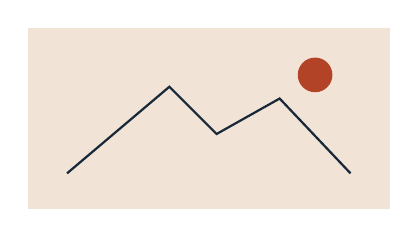
\begin{tikzpicture}[x=1cm,y=1cm]
      \fill[tint] (0,0) rectangle (4.6,2.3);
      \draw[ink,thick] (.5,.45) -- (1.8,1.55) -- (2.4,.95) -- (3.2,1.4) -- (4.1,.45);
      \fill[accent] (3.65,1.7) circle (2.2mm);
    \end{tikzpicture}
  \end{center}
  Replace the drawing with a photo or keep the page all text.
  \PageNo{02}
}
\ZinePage{3}{
  \Kicker{03 / PRINT}
  \Headline{One side only}
  Print the landscape sheet at \textbf{Actual Size (100\%)} on A4, or select US Letter in the source first.
  \medskip\par
  The top row is upside down on purpose.
  \PageNo{03}
}
\ZinePage{4}{
  \Kicker{04 / CREASE}
  \Headline{Make eight panels}
  Crease the sheet once down its length and three times across its width, following the dashed guides.
  \medskip\par
  Unfold it flat before making the cut.
  \PageNo{04}
}
\ZinePage{5}{
  \Kicker{05 / CUT}
  \Headline{Just one slit}
  Cut along the \textbf{solid middle line only}: start at the first vertical fold and stop at the third.
  \medskip\par
  Leave both outer sections attached.
  \PageNo{05}
}
\ZinePage{6}{
  \Kicker{06 / FOLD}
  \Headline{Push the ends in}
  Fold lengthwise with the print facing out. Push the two short ends toward each other until the slit opens into a diamond.
  \medskip\par
  Flatten the diamond into a cross, then wrap the panels until the front and back covers are on the outside.
  \PageNo{06}
}
\ZinePage{7}{
  \Kicker{BACK COVER}
  \vspace{15mm}
  {\sffamily\bfseries\LARGE Made to fold.\par}\medskip
  One sheet of paper.\par
  No staples or glue.\par
  \vspace{7mm}
  {\color{accent}\rule{20mm}{1.3pt}}
}

% ---- Imposition engine. You shouldn't need to edit below this line. ----
\newsavebox\PanelContent
\newcommand\PanelBox[1]{%
  \begin{lrbox}{\PanelContent}%
    \begin{minipage}{\InnerW}%
      \raggedright\normalfont\normalsize\color{ink}%
      \setlength\parskip{3pt}%
      \csname zinepage#1\endcsname\par
    \end{minipage}%
  \end{lrbox}%
  \ifdim\dimexpr\ht\PanelContent+\dp\PanelContent\relax>\InnerH
    \PackageWarningNoLine{mini-zine}{Panel #1 exceeds the safe height; shorten the content}%
  \fi
  \begin{minipage}[c][\InnerH][t]{\InnerW}%
    \noindent\usebox\PanelContent\par
  \end{minipage}%
}
\newcommand\ZineSheet{%
  \null
  \begin{tikzpicture}[remember picture,overlay]
    \begin{scope}[shift={(current page.south west)},x=\PanelW,y=\PanelH]
      % Printed view, left to right: 6 5 4 3 up top; back front 1 2 below.
      \foreach \p [count=\i from 0] in {7,0,1,2}
        \node[inner sep=0pt,outer sep=0pt] at ({\i+.5},.5) {\PanelBox{\p}};
      \foreach \p [count=\i from 0] in {6,5,4,3}
        \node[inner sep=0pt,outer sep=0pt,rotate=180] at ({\i+.5},1.5) {\PanelBox{\p}};
      \ifdefined\ZineNoGuides\else
        \foreach \x in {1,2,3}
          \draw[muted!60,dashed,line width=.3pt] ([yshift=5mm]\x,0) -- ([yshift=-5mm]\x,2);
        \draw[muted!60,dashed,line width=.3pt] ([xshift=5mm]0,1) -- (1,1);
        \draw[muted!60,dashed,line width=.3pt] (3,1) -- ([xshift=-5mm]4,1);
        \draw[accent,line width=.65pt] (1,1) -- (3,1);
      \fi
    \end{scope}
  \end{tikzpicture}%
}
\newcommand\ZineReadPage[1]{%
  \null
  \begin{tikzpicture}[remember picture,overlay]
    \node[inner sep=0pt,outer sep=0pt] at (current page.center) {\PanelBox{#1}};
  \end{tikzpicture}%
}

\begin{document}
\ifdefined\ZinePreview
  \ZineReadPage{0}\newpage\ZineReadPage{1}\newpage
  \ZineReadPage{2}\newpage\ZineReadPage{3}\newpage
  \ZineReadPage{4}\newpage\ZineReadPage{5}\newpage
  \ZineReadPage{6}\newpage\ZineReadPage{7}
\else
  \ZineSheet
\fi
\end{document}
"
% US Letter: uncomment \def\ZineLetter{1} below (or define it on the command line).
% Layout reference: https://github.com/krthr/fanzines.app#geometra-e-imposicin
% Print one-sided in landscape at Actual Size (100%), not "Fit".
% Crease the 4 x 2 grid. Cut ONLY the solid center segment between the
% first and third vertical folds. Fold lengthwise, print facing out, then
% push the two ends together; flatten the resulting cross into a booklet.
% \ZinePage{0} is the front, 1--6 are inside, and 7 is the back.
% Images: \includegraphics[width=\linewidth,height=30mm,keepaspectratio]{photo.jpg}

\RequirePackage{fix-cm}
\documentclass[10pt]{article}
\usepackage{geometry}
\usepackage{tikz}
\usepackage{graphicx}

% \def\ZineLetter{1}

\newlength\SheetW \newlength\SheetH
\newlength\PanelW \newlength\PanelH
\newlength\SafeMargin \setlength\SafeMargin{6mm}
\newlength\InnerW \newlength\InnerH
\ifdefined\ZineLetter
  \setlength\SheetW{11in} \setlength\SheetH{8.5in}
\else
  \setlength\SheetW{297mm} \setlength\SheetH{210mm}
\fi
\setlength\PanelW{\dimexpr\SheetW/4\relax}
\setlength\PanelH{\dimexpr\SheetH/2\relax}
\setlength\InnerW{\dimexpr\PanelW-2\SafeMargin\relax}
\setlength\InnerH{\dimexpr\PanelH-2\SafeMargin\relax}
\ifdefined\ZinePreview
  \geometry{paperwidth=\PanelW,paperheight=\PanelH,margin=0pt}
\else
  \geometry{paperwidth=\SheetW,paperheight=\SheetH,margin=0pt}
\fi
\pagestyle{empty}
\setlength\parindent{0pt}

\definecolor{ink}{HTML}{172839}
\definecolor{accent}{HTML}{B34327}
\definecolor{muted}{HTML}{545E6A}
\definecolor{tint}{HTML}{F1E3D6}

% ---- Edit these eight blocks, in reading order. ----
\newcommand\ZinePage[2]{\expandafter\long\expandafter\gdef\csname zinepage#1\endcsname{#2}}
\newcommand\Kicker[1]{\textcolor{accent}{\sffamily\bfseries\scriptsize #1}\par\smallskip}
\newcommand\Headline[1]{{\sffamily\bfseries\LARGE #1\par}\medskip}
\newcommand\PageNo[1]{\par\vspace{6mm}{\color{muted}\sffamily\scriptsize #1\par}}

\ZinePage{0}{
  \Kicker{A ONE-SHEET MINI-ZINE}
  \vspace{7mm}
  {\sffamily\bfseries\fontsize{27}{30}\selectfont
  One sheet.\par Eight pages.\par}
  \vspace{6mm}
  {\color{accent}\rule{20mm}{1.3pt}}\par\medskip
  Write it in order.\par Fold it into a book.
}
\ZinePage{1}{
  \Kicker{01 / WRITE}
  \Headline{Start here}
  Each page lives in a \texttt{\string\ZinePage} block. Write the cover, six inside pages, and the back in reading order.
  \medskip\par
  LaTeX takes care of flipping and rearranging them on the print sheet.
  \PageNo{01}
}
\ZinePage{2}{
  \Kicker{02 / DESIGN}
  \Headline{Make it yours}
  Use normal LaTeX: headings, lists, math, photos, or drawings.
  \begin{center}
    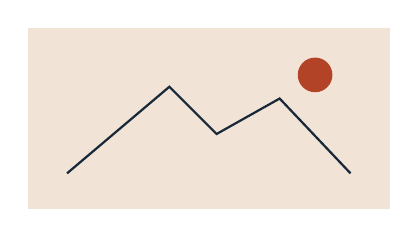
\begin{tikzpicture}[x=1cm,y=1cm]
      \fill[tint] (0,0) rectangle (4.6,2.3);
      \draw[ink,thick] (.5,.45) -- (1.8,1.55) -- (2.4,.95) -- (3.2,1.4) -- (4.1,.45);
      \fill[accent] (3.65,1.7) circle (2.2mm);
    \end{tikzpicture}
  \end{center}
  Replace the drawing with a photo or keep the page all text.
  \PageNo{02}
}
\ZinePage{3}{
  \Kicker{03 / PRINT}
  \Headline{One side only}
  Print the landscape sheet at \textbf{Actual Size (100\%)} on A4, or select US Letter in the source first.
  \medskip\par
  The top row is upside down on purpose.
  \PageNo{03}
}
\ZinePage{4}{
  \Kicker{04 / CREASE}
  \Headline{Make eight panels}
  Crease the sheet once down its length and three times across its width, following the dashed guides.
  \medskip\par
  Unfold it flat before making the cut.
  \PageNo{04}
}
\ZinePage{5}{
  \Kicker{05 / CUT}
  \Headline{Just one slit}
  Cut along the \textbf{solid middle line only}: start at the first vertical fold and stop at the third.
  \medskip\par
  Leave both outer sections attached.
  \PageNo{05}
}
\ZinePage{6}{
  \Kicker{06 / FOLD}
  \Headline{Push the ends in}
  Fold lengthwise with the print facing out. Push the two short ends toward each other until the slit opens into a diamond.
  \medskip\par
  Flatten the diamond into a cross, then wrap the panels until the front and back covers are on the outside.
  \PageNo{06}
}
\ZinePage{7}{
  \Kicker{BACK COVER}
  \vspace{15mm}
  {\sffamily\bfseries\LARGE Made to fold.\par}\medskip
  One sheet of paper.\par
  No staples or glue.\par
  \vspace{7mm}
  {\color{accent}\rule{20mm}{1.3pt}}
}

% ---- Imposition engine. You shouldn't need to edit below this line. ----
\newsavebox\PanelContent
\newcommand\PanelBox[1]{%
  \begin{lrbox}{\PanelContent}%
    \begin{minipage}{\InnerW}%
      \raggedright\normalfont\normalsize\color{ink}%
      \setlength\parskip{3pt}%
      \csname zinepage#1\endcsname\par
    \end{minipage}%
  \end{lrbox}%
  \ifdim\dimexpr\ht\PanelContent+\dp\PanelContent\relax>\InnerH
    \PackageWarningNoLine{mini-zine}{Panel #1 exceeds the safe height; shorten the content}%
  \fi
  \begin{minipage}[c][\InnerH][t]{\InnerW}%
    \noindent\usebox\PanelContent\par
  \end{minipage}%
}
\newcommand\ZineSheet{%
  \null
  \begin{tikzpicture}[remember picture,overlay]
    \begin{scope}[shift={(current page.south west)},x=\PanelW,y=\PanelH]
      % Printed view, left to right: 6 5 4 3 up top; back front 1 2 below.
      \foreach \p [count=\i from 0] in {7,0,1,2}
        \node[inner sep=0pt,outer sep=0pt] at ({\i+.5},.5) {\PanelBox{\p}};
      \foreach \p [count=\i from 0] in {6,5,4,3}
        \node[inner sep=0pt,outer sep=0pt,rotate=180] at ({\i+.5},1.5) {\PanelBox{\p}};
      \ifdefined\ZineNoGuides\else
        \foreach \x in {1,2,3}
          \draw[muted!60,dashed,line width=.3pt] ([yshift=5mm]\x,0) -- ([yshift=-5mm]\x,2);
        \draw[muted!60,dashed,line width=.3pt] ([xshift=5mm]0,1) -- (1,1);
        \draw[muted!60,dashed,line width=.3pt] (3,1) -- ([xshift=-5mm]4,1);
        \draw[accent,line width=.65pt] (1,1) -- (3,1);
      \fi
    \end{scope}
  \end{tikzpicture}%
}
\newcommand\ZineReadPage[1]{%
  \null
  \begin{tikzpicture}[remember picture,overlay]
    \node[inner sep=0pt,outer sep=0pt] at (current page.center) {\PanelBox{#1}};
  \end{tikzpicture}%
}

\begin{document}
\ifdefined\ZinePreview
  \ZineReadPage{0}\newpage\ZineReadPage{1}\newpage
  \ZineReadPage{2}\newpage\ZineReadPage{3}\newpage
  \ZineReadPage{4}\newpage\ZineReadPage{5}\newpage
  \ZineReadPage{6}\newpage\ZineReadPage{7}
\else
  \ZineSheet
\fi
\end{document}
"
% Clean:   pdflatex -jobname=mini-zine-clean "\def\ZineNoGuides{1}% ONE SHEET / EIGHT PAGES — single-file LaTeX mini-zine
% Print:   pdflatex mini-zine.tex  (run twice to resolve page positions)
% Preview: pdflatex -jobname=mini-zine-preview "\def\ZinePreview{1}% ONE SHEET / EIGHT PAGES — single-file LaTeX mini-zine
% Print:   pdflatex mini-zine.tex  (run twice to resolve page positions)
% Preview: pdflatex -jobname=mini-zine-preview "\def\ZinePreview{1}\input{mini-zine.tex}"
% Clean:   pdflatex -jobname=mini-zine-clean "\def\ZineNoGuides{1}\input{mini-zine.tex}"
% US Letter: uncomment \def\ZineLetter{1} below (or define it on the command line).
% Layout reference: https://github.com/krthr/fanzines.app#geometra-e-imposicin
% Print one-sided in landscape at Actual Size (100%), not "Fit".
% Crease the 4 x 2 grid. Cut ONLY the solid center segment between the
% first and third vertical folds. Fold lengthwise, print facing out, then
% push the two ends together; flatten the resulting cross into a booklet.
% \ZinePage{0} is the front, 1--6 are inside, and 7 is the back.
% Images: \includegraphics[width=\linewidth,height=30mm,keepaspectratio]{photo.jpg}

\RequirePackage{fix-cm}
\documentclass[10pt]{article}
\usepackage{geometry}
\usepackage{tikz}
\usepackage{graphicx}

% \def\ZineLetter{1}

\newlength\SheetW \newlength\SheetH
\newlength\PanelW \newlength\PanelH
\newlength\SafeMargin \setlength\SafeMargin{6mm}
\newlength\InnerW \newlength\InnerH
\ifdefined\ZineLetter
  \setlength\SheetW{11in} \setlength\SheetH{8.5in}
\else
  \setlength\SheetW{297mm} \setlength\SheetH{210mm}
\fi
\setlength\PanelW{\dimexpr\SheetW/4\relax}
\setlength\PanelH{\dimexpr\SheetH/2\relax}
\setlength\InnerW{\dimexpr\PanelW-2\SafeMargin\relax}
\setlength\InnerH{\dimexpr\PanelH-2\SafeMargin\relax}
\ifdefined\ZinePreview
  \geometry{paperwidth=\PanelW,paperheight=\PanelH,margin=0pt}
\else
  \geometry{paperwidth=\SheetW,paperheight=\SheetH,margin=0pt}
\fi
\pagestyle{empty}
\setlength\parindent{0pt}

\definecolor{ink}{HTML}{172839}
\definecolor{accent}{HTML}{B34327}
\definecolor{muted}{HTML}{545E6A}
\definecolor{tint}{HTML}{F1E3D6}

% ---- Edit these eight blocks, in reading order. ----
\newcommand\ZinePage[2]{\expandafter\long\expandafter\gdef\csname zinepage#1\endcsname{#2}}
\newcommand\Kicker[1]{\textcolor{accent}{\sffamily\bfseries\scriptsize #1}\par\smallskip}
\newcommand\Headline[1]{{\sffamily\bfseries\LARGE #1\par}\medskip}
\newcommand\PageNo[1]{\par\vspace{6mm}{\color{muted}\sffamily\scriptsize #1\par}}

\ZinePage{0}{
  \Kicker{A ONE-SHEET MINI-ZINE}
  \vspace{7mm}
  {\sffamily\bfseries\fontsize{27}{30}\selectfont
  One sheet.\par Eight pages.\par}
  \vspace{6mm}
  {\color{accent}\rule{20mm}{1.3pt}}\par\medskip
  Write it in order.\par Fold it into a book.
}
\ZinePage{1}{
  \Kicker{01 / WRITE}
  \Headline{Start here}
  Each page lives in a \texttt{\string\ZinePage} block. Write the cover, six inside pages, and the back in reading order.
  \medskip\par
  LaTeX takes care of flipping and rearranging them on the print sheet.
  \PageNo{01}
}
\ZinePage{2}{
  \Kicker{02 / DESIGN}
  \Headline{Make it yours}
  Use normal LaTeX: headings, lists, math, photos, or drawings.
  \begin{center}
    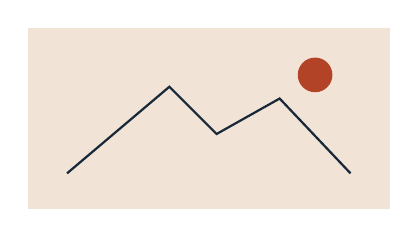
\begin{tikzpicture}[x=1cm,y=1cm]
      \fill[tint] (0,0) rectangle (4.6,2.3);
      \draw[ink,thick] (.5,.45) -- (1.8,1.55) -- (2.4,.95) -- (3.2,1.4) -- (4.1,.45);
      \fill[accent] (3.65,1.7) circle (2.2mm);
    \end{tikzpicture}
  \end{center}
  Replace the drawing with a photo or keep the page all text.
  \PageNo{02}
}
\ZinePage{3}{
  \Kicker{03 / PRINT}
  \Headline{One side only}
  Print the landscape sheet at \textbf{Actual Size (100\%)} on A4, or select US Letter in the source first.
  \medskip\par
  The top row is upside down on purpose.
  \PageNo{03}
}
\ZinePage{4}{
  \Kicker{04 / CREASE}
  \Headline{Make eight panels}
  Crease the sheet once down its length and three times across its width, following the dashed guides.
  \medskip\par
  Unfold it flat before making the cut.
  \PageNo{04}
}
\ZinePage{5}{
  \Kicker{05 / CUT}
  \Headline{Just one slit}
  Cut along the \textbf{solid middle line only}: start at the first vertical fold and stop at the third.
  \medskip\par
  Leave both outer sections attached.
  \PageNo{05}
}
\ZinePage{6}{
  \Kicker{06 / FOLD}
  \Headline{Push the ends in}
  Fold lengthwise with the print facing out. Push the two short ends toward each other until the slit opens into a diamond.
  \medskip\par
  Flatten the diamond into a cross, then wrap the panels until the front and back covers are on the outside.
  \PageNo{06}
}
\ZinePage{7}{
  \Kicker{BACK COVER}
  \vspace{15mm}
  {\sffamily\bfseries\LARGE Made to fold.\par}\medskip
  One sheet of paper.\par
  No staples or glue.\par
  \vspace{7mm}
  {\color{accent}\rule{20mm}{1.3pt}}
}

% ---- Imposition engine. You shouldn't need to edit below this line. ----
\newsavebox\PanelContent
\newcommand\PanelBox[1]{%
  \begin{lrbox}{\PanelContent}%
    \begin{minipage}{\InnerW}%
      \raggedright\normalfont\normalsize\color{ink}%
      \setlength\parskip{3pt}%
      \csname zinepage#1\endcsname\par
    \end{minipage}%
  \end{lrbox}%
  \ifdim\dimexpr\ht\PanelContent+\dp\PanelContent\relax>\InnerH
    \PackageWarningNoLine{mini-zine}{Panel #1 exceeds the safe height; shorten the content}%
  \fi
  \begin{minipage}[c][\InnerH][t]{\InnerW}%
    \noindent\usebox\PanelContent\par
  \end{minipage}%
}
\newcommand\ZineSheet{%
  \null
  \begin{tikzpicture}[remember picture,overlay]
    \begin{scope}[shift={(current page.south west)},x=\PanelW,y=\PanelH]
      % Printed view, left to right: 6 5 4 3 up top; back front 1 2 below.
      \foreach \p [count=\i from 0] in {7,0,1,2}
        \node[inner sep=0pt,outer sep=0pt] at ({\i+.5},.5) {\PanelBox{\p}};
      \foreach \p [count=\i from 0] in {6,5,4,3}
        \node[inner sep=0pt,outer sep=0pt,rotate=180] at ({\i+.5},1.5) {\PanelBox{\p}};
      \ifdefined\ZineNoGuides\else
        \foreach \x in {1,2,3}
          \draw[muted!60,dashed,line width=.3pt] ([yshift=5mm]\x,0) -- ([yshift=-5mm]\x,2);
        \draw[muted!60,dashed,line width=.3pt] ([xshift=5mm]0,1) -- (1,1);
        \draw[muted!60,dashed,line width=.3pt] (3,1) -- ([xshift=-5mm]4,1);
        \draw[accent,line width=.65pt] (1,1) -- (3,1);
      \fi
    \end{scope}
  \end{tikzpicture}%
}
\newcommand\ZineReadPage[1]{%
  \null
  \begin{tikzpicture}[remember picture,overlay]
    \node[inner sep=0pt,outer sep=0pt] at (current page.center) {\PanelBox{#1}};
  \end{tikzpicture}%
}

\begin{document}
\ifdefined\ZinePreview
  \ZineReadPage{0}\newpage\ZineReadPage{1}\newpage
  \ZineReadPage{2}\newpage\ZineReadPage{3}\newpage
  \ZineReadPage{4}\newpage\ZineReadPage{5}\newpage
  \ZineReadPage{6}\newpage\ZineReadPage{7}
\else
  \ZineSheet
\fi
\end{document}
"
% Clean:   pdflatex -jobname=mini-zine-clean "\def\ZineNoGuides{1}% ONE SHEET / EIGHT PAGES — single-file LaTeX mini-zine
% Print:   pdflatex mini-zine.tex  (run twice to resolve page positions)
% Preview: pdflatex -jobname=mini-zine-preview "\def\ZinePreview{1}\input{mini-zine.tex}"
% Clean:   pdflatex -jobname=mini-zine-clean "\def\ZineNoGuides{1}\input{mini-zine.tex}"
% US Letter: uncomment \def\ZineLetter{1} below (or define it on the command line).
% Layout reference: https://github.com/krthr/fanzines.app#geometra-e-imposicin
% Print one-sided in landscape at Actual Size (100%), not "Fit".
% Crease the 4 x 2 grid. Cut ONLY the solid center segment between the
% first and third vertical folds. Fold lengthwise, print facing out, then
% push the two ends together; flatten the resulting cross into a booklet.
% \ZinePage{0} is the front, 1--6 are inside, and 7 is the back.
% Images: \includegraphics[width=\linewidth,height=30mm,keepaspectratio]{photo.jpg}

\RequirePackage{fix-cm}
\documentclass[10pt]{article}
\usepackage{geometry}
\usepackage{tikz}
\usepackage{graphicx}

% \def\ZineLetter{1}

\newlength\SheetW \newlength\SheetH
\newlength\PanelW \newlength\PanelH
\newlength\SafeMargin \setlength\SafeMargin{6mm}
\newlength\InnerW \newlength\InnerH
\ifdefined\ZineLetter
  \setlength\SheetW{11in} \setlength\SheetH{8.5in}
\else
  \setlength\SheetW{297mm} \setlength\SheetH{210mm}
\fi
\setlength\PanelW{\dimexpr\SheetW/4\relax}
\setlength\PanelH{\dimexpr\SheetH/2\relax}
\setlength\InnerW{\dimexpr\PanelW-2\SafeMargin\relax}
\setlength\InnerH{\dimexpr\PanelH-2\SafeMargin\relax}
\ifdefined\ZinePreview
  \geometry{paperwidth=\PanelW,paperheight=\PanelH,margin=0pt}
\else
  \geometry{paperwidth=\SheetW,paperheight=\SheetH,margin=0pt}
\fi
\pagestyle{empty}
\setlength\parindent{0pt}

\definecolor{ink}{HTML}{172839}
\definecolor{accent}{HTML}{B34327}
\definecolor{muted}{HTML}{545E6A}
\definecolor{tint}{HTML}{F1E3D6}

% ---- Edit these eight blocks, in reading order. ----
\newcommand\ZinePage[2]{\expandafter\long\expandafter\gdef\csname zinepage#1\endcsname{#2}}
\newcommand\Kicker[1]{\textcolor{accent}{\sffamily\bfseries\scriptsize #1}\par\smallskip}
\newcommand\Headline[1]{{\sffamily\bfseries\LARGE #1\par}\medskip}
\newcommand\PageNo[1]{\par\vspace{6mm}{\color{muted}\sffamily\scriptsize #1\par}}

\ZinePage{0}{
  \Kicker{A ONE-SHEET MINI-ZINE}
  \vspace{7mm}
  {\sffamily\bfseries\fontsize{27}{30}\selectfont
  One sheet.\par Eight pages.\par}
  \vspace{6mm}
  {\color{accent}\rule{20mm}{1.3pt}}\par\medskip
  Write it in order.\par Fold it into a book.
}
\ZinePage{1}{
  \Kicker{01 / WRITE}
  \Headline{Start here}
  Each page lives in a \texttt{\string\ZinePage} block. Write the cover, six inside pages, and the back in reading order.
  \medskip\par
  LaTeX takes care of flipping and rearranging them on the print sheet.
  \PageNo{01}
}
\ZinePage{2}{
  \Kicker{02 / DESIGN}
  \Headline{Make it yours}
  Use normal LaTeX: headings, lists, math, photos, or drawings.
  \begin{center}
    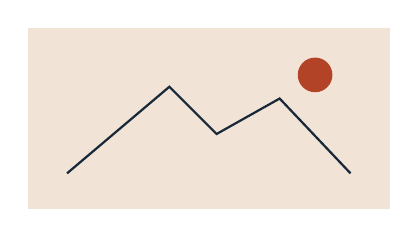
\begin{tikzpicture}[x=1cm,y=1cm]
      \fill[tint] (0,0) rectangle (4.6,2.3);
      \draw[ink,thick] (.5,.45) -- (1.8,1.55) -- (2.4,.95) -- (3.2,1.4) -- (4.1,.45);
      \fill[accent] (3.65,1.7) circle (2.2mm);
    \end{tikzpicture}
  \end{center}
  Replace the drawing with a photo or keep the page all text.
  \PageNo{02}
}
\ZinePage{3}{
  \Kicker{03 / PRINT}
  \Headline{One side only}
  Print the landscape sheet at \textbf{Actual Size (100\%)} on A4, or select US Letter in the source first.
  \medskip\par
  The top row is upside down on purpose.
  \PageNo{03}
}
\ZinePage{4}{
  \Kicker{04 / CREASE}
  \Headline{Make eight panels}
  Crease the sheet once down its length and three times across its width, following the dashed guides.
  \medskip\par
  Unfold it flat before making the cut.
  \PageNo{04}
}
\ZinePage{5}{
  \Kicker{05 / CUT}
  \Headline{Just one slit}
  Cut along the \textbf{solid middle line only}: start at the first vertical fold and stop at the third.
  \medskip\par
  Leave both outer sections attached.
  \PageNo{05}
}
\ZinePage{6}{
  \Kicker{06 / FOLD}
  \Headline{Push the ends in}
  Fold lengthwise with the print facing out. Push the two short ends toward each other until the slit opens into a diamond.
  \medskip\par
  Flatten the diamond into a cross, then wrap the panels until the front and back covers are on the outside.
  \PageNo{06}
}
\ZinePage{7}{
  \Kicker{BACK COVER}
  \vspace{15mm}
  {\sffamily\bfseries\LARGE Made to fold.\par}\medskip
  One sheet of paper.\par
  No staples or glue.\par
  \vspace{7mm}
  {\color{accent}\rule{20mm}{1.3pt}}
}

% ---- Imposition engine. You shouldn't need to edit below this line. ----
\newsavebox\PanelContent
\newcommand\PanelBox[1]{%
  \begin{lrbox}{\PanelContent}%
    \begin{minipage}{\InnerW}%
      \raggedright\normalfont\normalsize\color{ink}%
      \setlength\parskip{3pt}%
      \csname zinepage#1\endcsname\par
    \end{minipage}%
  \end{lrbox}%
  \ifdim\dimexpr\ht\PanelContent+\dp\PanelContent\relax>\InnerH
    \PackageWarningNoLine{mini-zine}{Panel #1 exceeds the safe height; shorten the content}%
  \fi
  \begin{minipage}[c][\InnerH][t]{\InnerW}%
    \noindent\usebox\PanelContent\par
  \end{minipage}%
}
\newcommand\ZineSheet{%
  \null
  \begin{tikzpicture}[remember picture,overlay]
    \begin{scope}[shift={(current page.south west)},x=\PanelW,y=\PanelH]
      % Printed view, left to right: 6 5 4 3 up top; back front 1 2 below.
      \foreach \p [count=\i from 0] in {7,0,1,2}
        \node[inner sep=0pt,outer sep=0pt] at ({\i+.5},.5) {\PanelBox{\p}};
      \foreach \p [count=\i from 0] in {6,5,4,3}
        \node[inner sep=0pt,outer sep=0pt,rotate=180] at ({\i+.5},1.5) {\PanelBox{\p}};
      \ifdefined\ZineNoGuides\else
        \foreach \x in {1,2,3}
          \draw[muted!60,dashed,line width=.3pt] ([yshift=5mm]\x,0) -- ([yshift=-5mm]\x,2);
        \draw[muted!60,dashed,line width=.3pt] ([xshift=5mm]0,1) -- (1,1);
        \draw[muted!60,dashed,line width=.3pt] (3,1) -- ([xshift=-5mm]4,1);
        \draw[accent,line width=.65pt] (1,1) -- (3,1);
      \fi
    \end{scope}
  \end{tikzpicture}%
}
\newcommand\ZineReadPage[1]{%
  \null
  \begin{tikzpicture}[remember picture,overlay]
    \node[inner sep=0pt,outer sep=0pt] at (current page.center) {\PanelBox{#1}};
  \end{tikzpicture}%
}

\begin{document}
\ifdefined\ZinePreview
  \ZineReadPage{0}\newpage\ZineReadPage{1}\newpage
  \ZineReadPage{2}\newpage\ZineReadPage{3}\newpage
  \ZineReadPage{4}\newpage\ZineReadPage{5}\newpage
  \ZineReadPage{6}\newpage\ZineReadPage{7}
\else
  \ZineSheet
\fi
\end{document}
"
% US Letter: uncomment \def\ZineLetter{1} below (or define it on the command line).
% Layout reference: https://github.com/krthr/fanzines.app#geometra-e-imposicin
% Print one-sided in landscape at Actual Size (100%), not "Fit".
% Crease the 4 x 2 grid. Cut ONLY the solid center segment between the
% first and third vertical folds. Fold lengthwise, print facing out, then
% push the two ends together; flatten the resulting cross into a booklet.
% \ZinePage{0} is the front, 1--6 are inside, and 7 is the back.
% Images: \includegraphics[width=\linewidth,height=30mm,keepaspectratio]{photo.jpg}

\RequirePackage{fix-cm}
\documentclass[10pt]{article}
\usepackage{geometry}
\usepackage{tikz}
\usepackage{graphicx}

% \def\ZineLetter{1}

\newlength\SheetW \newlength\SheetH
\newlength\PanelW \newlength\PanelH
\newlength\SafeMargin \setlength\SafeMargin{6mm}
\newlength\InnerW \newlength\InnerH
\ifdefined\ZineLetter
  \setlength\SheetW{11in} \setlength\SheetH{8.5in}
\else
  \setlength\SheetW{297mm} \setlength\SheetH{210mm}
\fi
\setlength\PanelW{\dimexpr\SheetW/4\relax}
\setlength\PanelH{\dimexpr\SheetH/2\relax}
\setlength\InnerW{\dimexpr\PanelW-2\SafeMargin\relax}
\setlength\InnerH{\dimexpr\PanelH-2\SafeMargin\relax}
\ifdefined\ZinePreview
  \geometry{paperwidth=\PanelW,paperheight=\PanelH,margin=0pt}
\else
  \geometry{paperwidth=\SheetW,paperheight=\SheetH,margin=0pt}
\fi
\pagestyle{empty}
\setlength\parindent{0pt}

\definecolor{ink}{HTML}{172839}
\definecolor{accent}{HTML}{B34327}
\definecolor{muted}{HTML}{545E6A}
\definecolor{tint}{HTML}{F1E3D6}

% ---- Edit these eight blocks, in reading order. ----
\newcommand\ZinePage[2]{\expandafter\long\expandafter\gdef\csname zinepage#1\endcsname{#2}}
\newcommand\Kicker[1]{\textcolor{accent}{\sffamily\bfseries\scriptsize #1}\par\smallskip}
\newcommand\Headline[1]{{\sffamily\bfseries\LARGE #1\par}\medskip}
\newcommand\PageNo[1]{\par\vspace{6mm}{\color{muted}\sffamily\scriptsize #1\par}}

\ZinePage{0}{
  \Kicker{A ONE-SHEET MINI-ZINE}
  \vspace{7mm}
  {\sffamily\bfseries\fontsize{27}{30}\selectfont
  One sheet.\par Eight pages.\par}
  \vspace{6mm}
  {\color{accent}\rule{20mm}{1.3pt}}\par\medskip
  Write it in order.\par Fold it into a book.
}
\ZinePage{1}{
  \Kicker{01 / WRITE}
  \Headline{Start here}
  Each page lives in a \texttt{\string\ZinePage} block. Write the cover, six inside pages, and the back in reading order.
  \medskip\par
  LaTeX takes care of flipping and rearranging them on the print sheet.
  \PageNo{01}
}
\ZinePage{2}{
  \Kicker{02 / DESIGN}
  \Headline{Make it yours}
  Use normal LaTeX: headings, lists, math, photos, or drawings.
  \begin{center}
    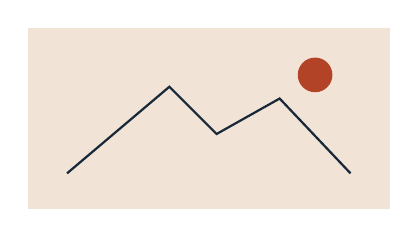
\begin{tikzpicture}[x=1cm,y=1cm]
      \fill[tint] (0,0) rectangle (4.6,2.3);
      \draw[ink,thick] (.5,.45) -- (1.8,1.55) -- (2.4,.95) -- (3.2,1.4) -- (4.1,.45);
      \fill[accent] (3.65,1.7) circle (2.2mm);
    \end{tikzpicture}
  \end{center}
  Replace the drawing with a photo or keep the page all text.
  \PageNo{02}
}
\ZinePage{3}{
  \Kicker{03 / PRINT}
  \Headline{One side only}
  Print the landscape sheet at \textbf{Actual Size (100\%)} on A4, or select US Letter in the source first.
  \medskip\par
  The top row is upside down on purpose.
  \PageNo{03}
}
\ZinePage{4}{
  \Kicker{04 / CREASE}
  \Headline{Make eight panels}
  Crease the sheet once down its length and three times across its width, following the dashed guides.
  \medskip\par
  Unfold it flat before making the cut.
  \PageNo{04}
}
\ZinePage{5}{
  \Kicker{05 / CUT}
  \Headline{Just one slit}
  Cut along the \textbf{solid middle line only}: start at the first vertical fold and stop at the third.
  \medskip\par
  Leave both outer sections attached.
  \PageNo{05}
}
\ZinePage{6}{
  \Kicker{06 / FOLD}
  \Headline{Push the ends in}
  Fold lengthwise with the print facing out. Push the two short ends toward each other until the slit opens into a diamond.
  \medskip\par
  Flatten the diamond into a cross, then wrap the panels until the front and back covers are on the outside.
  \PageNo{06}
}
\ZinePage{7}{
  \Kicker{BACK COVER}
  \vspace{15mm}
  {\sffamily\bfseries\LARGE Made to fold.\par}\medskip
  One sheet of paper.\par
  No staples or glue.\par
  \vspace{7mm}
  {\color{accent}\rule{20mm}{1.3pt}}
}

% ---- Imposition engine. You shouldn't need to edit below this line. ----
\newsavebox\PanelContent
\newcommand\PanelBox[1]{%
  \begin{lrbox}{\PanelContent}%
    \begin{minipage}{\InnerW}%
      \raggedright\normalfont\normalsize\color{ink}%
      \setlength\parskip{3pt}%
      \csname zinepage#1\endcsname\par
    \end{minipage}%
  \end{lrbox}%
  \ifdim\dimexpr\ht\PanelContent+\dp\PanelContent\relax>\InnerH
    \PackageWarningNoLine{mini-zine}{Panel #1 exceeds the safe height; shorten the content}%
  \fi
  \begin{minipage}[c][\InnerH][t]{\InnerW}%
    \noindent\usebox\PanelContent\par
  \end{minipage}%
}
\newcommand\ZineSheet{%
  \null
  \begin{tikzpicture}[remember picture,overlay]
    \begin{scope}[shift={(current page.south west)},x=\PanelW,y=\PanelH]
      % Printed view, left to right: 6 5 4 3 up top; back front 1 2 below.
      \foreach \p [count=\i from 0] in {7,0,1,2}
        \node[inner sep=0pt,outer sep=0pt] at ({\i+.5},.5) {\PanelBox{\p}};
      \foreach \p [count=\i from 0] in {6,5,4,3}
        \node[inner sep=0pt,outer sep=0pt,rotate=180] at ({\i+.5},1.5) {\PanelBox{\p}};
      \ifdefined\ZineNoGuides\else
        \foreach \x in {1,2,3}
          \draw[muted!60,dashed,line width=.3pt] ([yshift=5mm]\x,0) -- ([yshift=-5mm]\x,2);
        \draw[muted!60,dashed,line width=.3pt] ([xshift=5mm]0,1) -- (1,1);
        \draw[muted!60,dashed,line width=.3pt] (3,1) -- ([xshift=-5mm]4,1);
        \draw[accent,line width=.65pt] (1,1) -- (3,1);
      \fi
    \end{scope}
  \end{tikzpicture}%
}
\newcommand\ZineReadPage[1]{%
  \null
  \begin{tikzpicture}[remember picture,overlay]
    \node[inner sep=0pt,outer sep=0pt] at (current page.center) {\PanelBox{#1}};
  \end{tikzpicture}%
}

\begin{document}
\ifdefined\ZinePreview
  \ZineReadPage{0}\newpage\ZineReadPage{1}\newpage
  \ZineReadPage{2}\newpage\ZineReadPage{3}\newpage
  \ZineReadPage{4}\newpage\ZineReadPage{5}\newpage
  \ZineReadPage{6}\newpage\ZineReadPage{7}
\else
  \ZineSheet
\fi
\end{document}
"
% US Letter: uncomment \def\ZineLetter{1} below (or define it on the command line).
% Layout reference: https://github.com/krthr/fanzines.app#geometra-e-imposicin
% Print one-sided in landscape at Actual Size (100%), not "Fit".
% Crease the 4 x 2 grid. Cut ONLY the solid center segment between the
% first and third vertical folds. Fold lengthwise, print facing out, then
% push the two ends together; flatten the resulting cross into a booklet.
% \ZinePage{0} is the front, 1--6 are inside, and 7 is the back.
% Images: \includegraphics[width=\linewidth,height=30mm,keepaspectratio]{photo.jpg}

\RequirePackage{fix-cm}
\documentclass[10pt]{article}
\usepackage{geometry}
\usepackage{tikz}
\usepackage{graphicx}

% \def\ZineLetter{1}

\newlength\SheetW \newlength\SheetH
\newlength\PanelW \newlength\PanelH
\newlength\SafeMargin \setlength\SafeMargin{6mm}
\newlength\InnerW \newlength\InnerH
\ifdefined\ZineLetter
  \setlength\SheetW{11in} \setlength\SheetH{8.5in}
\else
  \setlength\SheetW{297mm} \setlength\SheetH{210mm}
\fi
\setlength\PanelW{\dimexpr\SheetW/4\relax}
\setlength\PanelH{\dimexpr\SheetH/2\relax}
\setlength\InnerW{\dimexpr\PanelW-2\SafeMargin\relax}
\setlength\InnerH{\dimexpr\PanelH-2\SafeMargin\relax}
\ifdefined\ZinePreview
  \geometry{paperwidth=\PanelW,paperheight=\PanelH,margin=0pt}
\else
  \geometry{paperwidth=\SheetW,paperheight=\SheetH,margin=0pt}
\fi
\pagestyle{empty}
\setlength\parindent{0pt}

\definecolor{ink}{HTML}{172839}
\definecolor{accent}{HTML}{B34327}
\definecolor{muted}{HTML}{545E6A}
\definecolor{tint}{HTML}{F1E3D6}

% ---- Edit these eight blocks, in reading order. ----
\newcommand\ZinePage[2]{\expandafter\long\expandafter\gdef\csname zinepage#1\endcsname{#2}}
\newcommand\Kicker[1]{\textcolor{accent}{\sffamily\bfseries\scriptsize #1}\par\smallskip}
\newcommand\Headline[1]{{\sffamily\bfseries\LARGE #1\par}\medskip}
\newcommand\PageNo[1]{\par\vspace{6mm}{\color{muted}\sffamily\scriptsize #1\par}}

\ZinePage{0}{
  \Kicker{A ONE-SHEET MINI-ZINE}
  \vspace{7mm}
  {\sffamily\bfseries\fontsize{27}{30}\selectfont
  One sheet.\par Eight pages.\par}
  \vspace{6mm}
  {\color{accent}\rule{20mm}{1.3pt}}\par\medskip
  Write it in order.\par Fold it into a book.
}
\ZinePage{1}{
  \Kicker{01 / WRITE}
  \Headline{Start here}
  Each page lives in a \texttt{\string\ZinePage} block. Write the cover, six inside pages, and the back in reading order.
  \medskip\par
  LaTeX takes care of flipping and rearranging them on the print sheet.
  \PageNo{01}
}
\ZinePage{2}{
  \Kicker{02 / DESIGN}
  \Headline{Make it yours}
  Use normal LaTeX: headings, lists, math, photos, or drawings.
  \begin{center}
    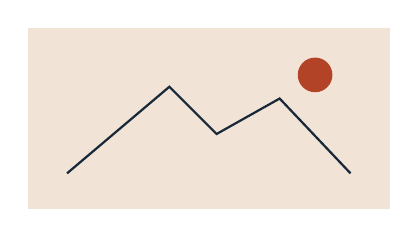
\begin{tikzpicture}[x=1cm,y=1cm]
      \fill[tint] (0,0) rectangle (4.6,2.3);
      \draw[ink,thick] (.5,.45) -- (1.8,1.55) -- (2.4,.95) -- (3.2,1.4) -- (4.1,.45);
      \fill[accent] (3.65,1.7) circle (2.2mm);
    \end{tikzpicture}
  \end{center}
  Replace the drawing with a photo or keep the page all text.
  \PageNo{02}
}
\ZinePage{3}{
  \Kicker{03 / PRINT}
  \Headline{One side only}
  Print the landscape sheet at \textbf{Actual Size (100\%)} on A4, or select US Letter in the source first.
  \medskip\par
  The top row is upside down on purpose.
  \PageNo{03}
}
\ZinePage{4}{
  \Kicker{04 / CREASE}
  \Headline{Make eight panels}
  Crease the sheet once down its length and three times across its width, following the dashed guides.
  \medskip\par
  Unfold it flat before making the cut.
  \PageNo{04}
}
\ZinePage{5}{
  \Kicker{05 / CUT}
  \Headline{Just one slit}
  Cut along the \textbf{solid middle line only}: start at the first vertical fold and stop at the third.
  \medskip\par
  Leave both outer sections attached.
  \PageNo{05}
}
\ZinePage{6}{
  \Kicker{06 / FOLD}
  \Headline{Push the ends in}
  Fold lengthwise with the print facing out. Push the two short ends toward each other until the slit opens into a diamond.
  \medskip\par
  Flatten the diamond into a cross, then wrap the panels until the front and back covers are on the outside.
  \PageNo{06}
}
\ZinePage{7}{
  \Kicker{BACK COVER}
  \vspace{15mm}
  {\sffamily\bfseries\LARGE Made to fold.\par}\medskip
  One sheet of paper.\par
  No staples or glue.\par
  \vspace{7mm}
  {\color{accent}\rule{20mm}{1.3pt}}
}

% ---- Imposition engine. You shouldn't need to edit below this line. ----
\newsavebox\PanelContent
\newcommand\PanelBox[1]{%
  \begin{lrbox}{\PanelContent}%
    \begin{minipage}{\InnerW}%
      \raggedright\normalfont\normalsize\color{ink}%
      \setlength\parskip{3pt}%
      \csname zinepage#1\endcsname\par
    \end{minipage}%
  \end{lrbox}%
  \ifdim\dimexpr\ht\PanelContent+\dp\PanelContent\relax>\InnerH
    \PackageWarningNoLine{mini-zine}{Panel #1 exceeds the safe height; shorten the content}%
  \fi
  \begin{minipage}[c][\InnerH][t]{\InnerW}%
    \noindent\usebox\PanelContent\par
  \end{minipage}%
}
\newcommand\ZineSheet{%
  \null
  \begin{tikzpicture}[remember picture,overlay]
    \begin{scope}[shift={(current page.south west)},x=\PanelW,y=\PanelH]
      % Printed view, left to right: 6 5 4 3 up top; back front 1 2 below.
      \foreach \p [count=\i from 0] in {7,0,1,2}
        \node[inner sep=0pt,outer sep=0pt] at ({\i+.5},.5) {\PanelBox{\p}};
      \foreach \p [count=\i from 0] in {6,5,4,3}
        \node[inner sep=0pt,outer sep=0pt,rotate=180] at ({\i+.5},1.5) {\PanelBox{\p}};
      \ifdefined\ZineNoGuides\else
        \foreach \x in {1,2,3}
          \draw[muted!60,dashed,line width=.3pt] ([yshift=5mm]\x,0) -- ([yshift=-5mm]\x,2);
        \draw[muted!60,dashed,line width=.3pt] ([xshift=5mm]0,1) -- (1,1);
        \draw[muted!60,dashed,line width=.3pt] (3,1) -- ([xshift=-5mm]4,1);
        \draw[accent,line width=.65pt] (1,1) -- (3,1);
      \fi
    \end{scope}
  \end{tikzpicture}%
}
\newcommand\ZineReadPage[1]{%
  \null
  \begin{tikzpicture}[remember picture,overlay]
    \node[inner sep=0pt,outer sep=0pt] at (current page.center) {\PanelBox{#1}};
  \end{tikzpicture}%
}

\begin{document}
\ifdefined\ZinePreview
  \ZineReadPage{0}\newpage\ZineReadPage{1}\newpage
  \ZineReadPage{2}\newpage\ZineReadPage{3}\newpage
  \ZineReadPage{4}\newpage\ZineReadPage{5}\newpage
  \ZineReadPage{6}\newpage\ZineReadPage{7}
\else
  \ZineSheet
\fi
\end{document}
"
% US Letter: uncomment \def\ZineLetter{1} below (or define it on the command line).
% Layout reference: https://github.com/krthr/fanzines.app#geometra-e-imposicin
% Print one-sided in landscape at Actual Size (100%), not "Fit".
% Crease the 4 x 2 grid. Cut ONLY the solid center segment between the
% first and third vertical folds. Fold lengthwise, print facing out, then
% push the two ends together; flatten the resulting cross into a booklet.
% \ZinePage{0} is the front, 1--6 are inside, and 7 is the back.
% Images: \includegraphics[width=\linewidth,height=30mm,keepaspectratio]{photo.jpg}

\RequirePackage{fix-cm}
\documentclass[10pt]{article}
\usepackage{geometry}
\usepackage{tikz}
\usepackage{graphicx}

% \def\ZineLetter{1}

\newlength\SheetW \newlength\SheetH
\newlength\PanelW \newlength\PanelH
\newlength\SafeMargin \setlength\SafeMargin{6mm}
\newlength\InnerW \newlength\InnerH
\ifdefined\ZineLetter
  \setlength\SheetW{11in} \setlength\SheetH{8.5in}
\else
  \setlength\SheetW{297mm} \setlength\SheetH{210mm}
\fi
\setlength\PanelW{\dimexpr\SheetW/4\relax}
\setlength\PanelH{\dimexpr\SheetH/2\relax}
\setlength\InnerW{\dimexpr\PanelW-2\SafeMargin\relax}
\setlength\InnerH{\dimexpr\PanelH-2\SafeMargin\relax}
\ifdefined\ZinePreview
  \geometry{paperwidth=\PanelW,paperheight=\PanelH,margin=0pt}
\else
  \geometry{paperwidth=\SheetW,paperheight=\SheetH,margin=0pt}
\fi
\pagestyle{empty}
\setlength\parindent{0pt}

\definecolor{ink}{HTML}{172839}
\definecolor{accent}{HTML}{B34327}
\definecolor{muted}{HTML}{545E6A}
\definecolor{tint}{HTML}{F1E3D6}

% ---- Edit these eight blocks, in reading order. ----
\newcommand\ZinePage[2]{\expandafter\long\expandafter\gdef\csname zinepage#1\endcsname{#2}}
\newcommand\Kicker[1]{\textcolor{accent}{\sffamily\bfseries\scriptsize #1}\par\smallskip}
\newcommand\Headline[1]{{\sffamily\bfseries\LARGE #1\par}\medskip}
\newcommand\PageNo[1]{\par\vspace{6mm}{\color{muted}\sffamily\scriptsize #1\par}}

\ZinePage{0}{
  \Kicker{A ONE-SHEET MINI-ZINE}
  \vspace{7mm}
  {\sffamily\bfseries\fontsize{27}{30}\selectfont
  One sheet.\par Eight pages.\par}
  \vspace{6mm}
  {\color{accent}\rule{20mm}{1.3pt}}\par\medskip
  Write it in order.\par Fold it into a book.
}
\ZinePage{1}{
  \Kicker{01 / WRITE}
  \Headline{Start here}
  Each page lives in a \texttt{\string\ZinePage} block. Write the cover, six inside pages, and the back in reading order.
  \medskip\par
  LaTeX takes care of flipping and rearranging them on the print sheet.
  \PageNo{01}
}
\ZinePage{2}{
  \Kicker{02 / DESIGN}
  \Headline{Make it yours}
  Use normal LaTeX: headings, lists, math, photos, or drawings.
  \begin{center}
    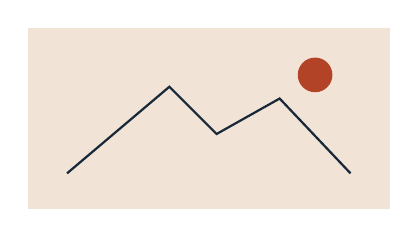
\begin{tikzpicture}[x=1cm,y=1cm]
      \fill[tint] (0,0) rectangle (4.6,2.3);
      \draw[ink,thick] (.5,.45) -- (1.8,1.55) -- (2.4,.95) -- (3.2,1.4) -- (4.1,.45);
      \fill[accent] (3.65,1.7) circle (2.2mm);
    \end{tikzpicture}
  \end{center}
  Replace the drawing with a photo or keep the page all text.
  \PageNo{02}
}
\ZinePage{3}{
  \Kicker{03 / PRINT}
  \Headline{One side only}
  Print the landscape sheet at \textbf{Actual Size (100\%)} on A4, or select US Letter in the source first.
  \medskip\par
  The top row is upside down on purpose.
  \PageNo{03}
}
\ZinePage{4}{
  \Kicker{04 / CREASE}
  \Headline{Make eight panels}
  Crease the sheet once down its length and three times across its width, following the dashed guides.
  \medskip\par
  Unfold it flat before making the cut.
  \PageNo{04}
}
\ZinePage{5}{
  \Kicker{05 / CUT}
  \Headline{Just one slit}
  Cut along the \textbf{solid middle line only}: start at the first vertical fold and stop at the third.
  \medskip\par
  Leave both outer sections attached.
  \PageNo{05}
}
\ZinePage{6}{
  \Kicker{06 / FOLD}
  \Headline{Push the ends in}
  Fold lengthwise with the print facing out. Push the two short ends toward each other until the slit opens into a diamond.
  \medskip\par
  Flatten the diamond into a cross, then wrap the panels until the front and back covers are on the outside.
  \PageNo{06}
}
\ZinePage{7}{
  \Kicker{BACK COVER}
  \vspace{15mm}
  {\sffamily\bfseries\LARGE Made to fold.\par}\medskip
  One sheet of paper.\par
  No staples or glue.\par
  \vspace{7mm}
  {\color{accent}\rule{20mm}{1.3pt}}
}

% ---- Imposition engine. You shouldn't need to edit below this line. ----
\newsavebox\PanelContent
\newcommand\PanelBox[1]{%
  \begin{lrbox}{\PanelContent}%
    \begin{minipage}{\InnerW}%
      \raggedright\normalfont\normalsize\color{ink}%
      \setlength\parskip{3pt}%
      \csname zinepage#1\endcsname\par
    \end{minipage}%
  \end{lrbox}%
  \ifdim\dimexpr\ht\PanelContent+\dp\PanelContent\relax>\InnerH
    \PackageWarningNoLine{mini-zine}{Panel #1 exceeds the safe height; shorten the content}%
  \fi
  \begin{minipage}[c][\InnerH][t]{\InnerW}%
    \noindent\usebox\PanelContent\par
  \end{minipage}%
}
\newcommand\ZineSheet{%
  \null
  \begin{tikzpicture}[remember picture,overlay]
    \begin{scope}[shift={(current page.south west)},x=\PanelW,y=\PanelH]
      % Printed view, left to right: 6 5 4 3 up top; back front 1 2 below.
      \foreach \p [count=\i from 0] in {7,0,1,2}
        \node[inner sep=0pt,outer sep=0pt] at ({\i+.5},.5) {\PanelBox{\p}};
      \foreach \p [count=\i from 0] in {6,5,4,3}
        \node[inner sep=0pt,outer sep=0pt,rotate=180] at ({\i+.5},1.5) {\PanelBox{\p}};
      \ifdefined\ZineNoGuides\else
        \foreach \x in {1,2,3}
          \draw[muted!60,dashed,line width=.3pt] ([yshift=5mm]\x,0) -- ([yshift=-5mm]\x,2);
        \draw[muted!60,dashed,line width=.3pt] ([xshift=5mm]0,1) -- (1,1);
        \draw[muted!60,dashed,line width=.3pt] (3,1) -- ([xshift=-5mm]4,1);
        \draw[accent,line width=.65pt] (1,1) -- (3,1);
      \fi
    \end{scope}
  \end{tikzpicture}%
}
\newcommand\ZineReadPage[1]{%
  \null
  \begin{tikzpicture}[remember picture,overlay]
    \node[inner sep=0pt,outer sep=0pt] at (current page.center) {\PanelBox{#1}};
  \end{tikzpicture}%
}

\begin{document}
\ifdefined\ZinePreview
  \ZineReadPage{0}\newpage\ZineReadPage{1}\newpage
  \ZineReadPage{2}\newpage\ZineReadPage{3}\newpage
  \ZineReadPage{4}\newpage\ZineReadPage{5}\newpage
  \ZineReadPage{6}\newpage\ZineReadPage{7}
\else
  \ZineSheet
\fi
\end{document}
